\documentclass[a4paper,12pt,twoside]{memoir}

% Castellano
\usepackage[spanish,es-tabla]{babel}
\selectlanguage{spanish}
\usepackage[utf8]{inputenc}
\usepackage[T1]{fontenc}
\usepackage{lmodern} % Scalable font
\usepackage{microtype}
\usepackage{placeins}

\RequirePackage{booktabs}
\RequirePackage[table]{xcolor}
\RequirePackage{xtab}
\RequirePackage{multirow}

% Links
\PassOptionsToPackage{hyphens}{url}\usepackage[colorlinks]{hyperref}
\hypersetup{
	allcolors = {red}
}

% Ecuaciones
\usepackage{amsmath}

% Rutas de fichero / paquete
\newcommand{\ruta}[1]{{\sffamily #1}}

% Párrafos
\nonzeroparskip

% Huérfanas y viudas
\widowpenalty100000
\clubpenalty100000

% Imagenes
\usepackage{graphicx}
\newcommand{\imagen}[2]{
	\begin{figure}[!h]
		\centering
		\includegraphics[width=0.9\textwidth]{#1}
		\caption{#2}\label{fig:#1}
	\end{figure}
	\FloatBarrier
}

\newcommand{\imagenflotante}[2]{
	\begin{figure}%[!h]
		\centering
		\includegraphics[width=0.9\textwidth]{#1}
		\caption{#2}\label{fig:#1}
	\end{figure}
}



% El comando \figura nos permite insertar figuras comodamente, y utilizando
% siempre el mismo formato. Los parametros son:
% 1 -> Porcentaje del ancho de página que ocupará la figura (de 0 a 1)
% 2 --> Fichero de la imagen
% 3 --> Texto a pie de imagen
% 4 --> Etiqueta (label) para referencias
% 5 --> Opciones que queramos pasarle al \includegraphics
% 6 --> Opciones de posicionamiento a pasarle a \begin{figure}
	\newcommand{\figuraConPosicion}[6]{%
		\setlength{\anchoFloat}{#1\textwidth}%
		\addtolength{\anchoFloat}{-4\fboxsep}%
		\setlength{\anchoFigura}{\anchoFloat}%
		\begin{figure}[#6]
			\begin{center}%
				\Ovalbox{%
					\begin{minipage}{\anchoFloat}%
						\begin{center}%
							\includegraphics[width=\anchoFigura,#5]{#2}%
							\caption{#3}%
							\label{#4}%
						\end{center}%
					\end{minipage}
				}%
			\end{center}%
		\end{figure}%
	}
	
	%
	% Comando para incluir imágenes en formato apaisado (sin marco).
	\newcommand{\figuraApaisadaSinMarco}[5]{%
		\begin{figure}%
			\begin{center}%
				\includegraphics[angle=90,height=#1\textheight,#5]{#2}%
				\caption{#3}%
				\label{#4}%
			\end{center}%
		\end{figure}%
	}
	% Para las tablas
	\newcommand{\otoprule}{\midrule [\heavyrulewidth]}
	%
	% Nuevo comando para tablas pequeñas (menos de una página).
	\newcommand{\tablaSmall}[5]{%
		\begin{table}
			\begin{center}
				\rowcolors {2}{gray!35}{}
				\begin{tabular}{#2}
					\toprule
					#4
					\otoprule
					#5
					\bottomrule
				\end{tabular}
				\caption{#1}
				\label{tabla:#3}
			\end{center}
		\end{table}
	}
	
	%
	% Nuevo comando para tablas pequeñas (menos de una página).
	\newcommand{\tablaSmallSinColores}[5]{%
		\begin{table}[H]
			\begin{center}
				\begin{tabular}{#2}
					\toprule
					#4
					\otoprule
					#5
					\bottomrule
				\end{tabular}
				\caption{#1}
				\label{tabla:#3}
			\end{center}
		\end{table}
	}
	
	\newcommand{\tablaApaisadaSmall}[5]{%
		\begin{landscape}
			\begin{table}
				\begin{center}
					\rowcolors {2}{gray!35}{}
					\begin{tabular}{#2}
						\toprule
						#4
						\otoprule
						#5
						\bottomrule
					\end{tabular}
					\caption{#1}
					\label{tabla:#3}
				\end{center}
			\end{table}
		\end{landscape}
	}
	
	%
	% Nuevo comando para tablas grandes con cabecera y filas alternas coloreadas en gris.
	\newcommand{\tabla}[6]{%
		\begin{center}
			\tablefirsthead{
				\toprule
				#5
				\otoprule
			}
			\tablehead{
				\multicolumn{#3}{l}{\small\sl continúa desde la página anterior}\\
				\toprule
				#5
				\otoprule
			}
			\tabletail{
				\hline
				\multicolumn{#3}{r}{\small\sl continúa en la página siguiente}\\
			}
			\tablelasttail{
				\hline
			}
			\bottomcaption{#1}
			\rowcolors {2}{gray!35}{}
			\begin{xtabular}{#2}
				#6
				\bottomrule
			\end{xtabular}
			\label{tabla:#4}
		\end{center}
	}
	
	%
	% Nuevo comando para tablas grandes con cabecera.
	\newcommand{\tablaSinColores}[6]{%
		\begin{center}
			\tablefirsthead{
				\toprule
				#5
				\otoprule
			}
			\tablehead{
				\multicolumn{#3}{l}{\small\sl continúa desde la página anterior}\\
				\toprule
				#5
				\otoprule
			}
			\tabletail{
				\hline
				\multicolumn{#3}{r}{\small\sl continúa en la página siguiente}\\
			}
			\tablelasttail{
				\hline
			}
			\bottomcaption{#1}
			\begin{xtabular}{#2}
				#6
				\bottomrule
			\end{xtabular}
			\label{tabla:#4}
		\end{center}
	}
	
	%
	% Nuevo comando para tablas grandes sin cabecera.
	\newcommand{\tablaSinCabecera}[5]{%
		\begin{center}
			\tablefirsthead{
				\toprule
			}
			\tablehead{
				\multicolumn{#3}{l}{\small\sl continúa desde la página anterior}\\
				\hline
			}
			\tabletail{
				\hline
				\multicolumn{#3}{r}{\small\sl continúa en la página siguiente}\\
			}
			\tablelasttail{
				\hline
			}
			\bottomcaption{#1}
			\begin{xtabular}{#2}
				#5
				\bottomrule
			\end{xtabular}
			\label{tabla:#4}
		\end{center}
	}
	
	
	
	\definecolor{cgoLight}{HTML}{EEEEEE}
	\definecolor{cgoExtralight}{HTML}{FFFFFF}
	
	%
	% Nuevo comando para tablas grandes sin cabecera.
	\newcommand{\tablaSinCabeceraConBandas}[5]{%
		\begin{center}
			\tablefirsthead{
				\toprule
			}
			\tablehead{
				\multicolumn{#3}{l}{\small\sl continúa desde la página anterior}\\
				\hline
			}
			\tabletail{
				\hline
				\multicolumn{#3}{r}{\small\sl continúa en la página siguiente}\\
			}
			\tablelasttail{
				\hline
			}
			\bottomcaption{#1}
			\rowcolors[]{1}{cgoExtralight}{cgoLight}
			
			\begin{xtabular}{#2}
				#5
				\bottomrule
			\end{xtabular}
			\label{tabla:#4}
		\end{center}
	}
	
	
	
	\graphicspath{ {./img/} }
	
	% Capítulos
	\chapterstyle{bianchi}
	\newcommand{\capitulo}[2]{
		\setcounter{chapter}{#1}
		\setcounter{section}{0}
		\setcounter{figure}{0}
		\setcounter{table}{0}
		\chapter*{#2}
		\addcontentsline{toc}{chapter}{#2}
		\markboth{#2}{#2}
	}
	
	% Apéndices
	\renewcommand{\appendixname}{Apéndice}
	\renewcommand*\cftappendixname{\appendixname}
	
	\newcommand{\apendice}[1]{
		%\renewcommand{\thechapter}{A}
		\chapter{#1}
	}
	
	\renewcommand*\cftappendixname{\appendixname\ }
	
	% Formato de portada
	\makeatletter
	\usepackage{xcolor}
	\newcommand{\tutor}[1]{\def\@tutor{#1}}
	\newcommand{\course}[1]{\def\@course{#1}}
	\definecolor{cpardoBox}{HTML}{E6E6FF}
	\def\maketitle{
		\null
		\thispagestyle{empty}
		% Cabecera ----------------
		\noindent\includegraphics[width=\textwidth]{cabecera}\vspace{1cm}%
		\vfill
		% Título proyecto y escudo informática ----------------
		\colorbox{cpardoBox}{%
			\begin{minipage}{.8\textwidth}
				\vspace{.5cm}\Large
				\begin{center}
					\textbf{TFG del Grado en Ingeniería Informática}\vspace{.6cm}\\
					\textbf{\LARGE\@title{}}
				\end{center}
				\vspace{.2cm}
			\end{minipage}
			
		}%
		\hfill\begin{minipage}{.20\textwidth}
			\includegraphics[width=\textwidth]{escudoInfor}
		\end{minipage}
		\vfill
		% Datos de alumno, curso y tutores ------------------
		\begin{center}%
			{%
				\noindent\LARGE
				Presentado por \@author{}\\ 
				en Universidad de Burgos --- \@date{}\\
				Tutores: \@tutor{}\\
			}%
		\end{center}%
		\null
		\cleardoublepage
	}
	\makeatother
	
	\newcommand{\nombre}{Álvaro Alonso Marín} %%% cambio de comando
	
	% Datos de portada
	\title{Identificación de Parkinson mediante visión artificial}
	\author{\nombre}
	\tutor{Álvar Arnaiz González y Alicia Olivares Gil}
	\date{\today}
	
	\begin{document}
		
		\maketitle
		
		
		\newpage\null\thispagestyle{empty}\newpage
		
		
		%%%%%%%%%%%%%%%%%%%%%%%%%%%%%%%%%%%%%%%%%%%%%%%%%%%%%%%%%%%%%%%%%%%%%%%%%%%%%%%%%%%%%%%%
		\thispagestyle{empty}
		
		
		\noindent\includegraphics[width=\textwidth]{cabecera}\vspace{1cm}
		
		\noindent Dña. Alicia Olivares Gil, profesora del departamento de Ingeniería Informática, área de Lenguajes y Sistemas Informáticos.
		
		\noindent Expone:
		
		\noindent Que el alumno D. \nombre, con DNI 71307942F, ha realizado el Trabajo final de Grado en Ingeniería Informática titulado Identificación de Parkinson mediante visión artificial. 
		
		\noindent Y que dicho trabajo ha sido realizado por el alumno bajo la dirección de la que suscribe, en virtud de lo cual se autoriza su presentación y defensa.
		
		\begin{center} %\large
			En Burgos, {\large \today}
		\end{center}
		
		\vfill\vfill\vfill
		
		% Author and supervisor
		\begin{minipage}{0.45\textwidth}
			\begin{flushleft} %\large
				Vº. Bº. del Tutor:\\[2cm]
				Dña. Alicia Olivares Gil
			\end{flushleft}
		\end{minipage}
		\hfill
		\begin{minipage}{0.45\textwidth}
			\begin{flushleft} %\large
				Vº. Bº. del co-tutor:\\[2cm]
				D. Álvar Arnaiz González
			\end{flushleft}
		\end{minipage}
		\hfill
		
		\vfill
		
		% para casos con solo un tutor comentar lo anterior
		% y descomentar lo siguiente
		%Vº. Bº. del Tutor:\\[2cm]
		%D. nombre tutor
		
		
		\newpage\null\thispagestyle{empty}\newpage
		
		
		
		
		\frontmatter
		
		% Abstract en castellano
		\renewcommand*\abstractname{Resumen}
		\begin{abstract}
		\end{abstract}
		
		\renewcommand*\abstractname{Descriptores}
		\begin{abstract}
		\end{abstract}
		
		\clearpage
		
		% Abstract en inglés
		\renewcommand*\abstractname{Abstract}
		\begin{abstract}
		\end{abstract}
		
		\renewcommand*\abstractname{Keywords}
		\begin{abstract}
		\end{abstract}
		
		\clearpage
		
		% Indices
		\tableofcontents
		
		\clearpage
		
		\listoffigures
		
		\clearpage
		
		\listoftables
		\clearpage
		
		\mainmatter
		\capitulo{1}{Introducción}
El Parkinson~\cite{parkinson} es una enfermedad neurodegenerativa crónica, la cual tiene síntomas como el aumento del tono muscular~\cite{tonomuscular} (contracción parcial, pasiva y continua de los músculos) y temblores.

Destaca como trastorno de movimiento, aunque también afecta a la función cognitiva, a la aparición de depresión y dolores, y a la función del sistema nervioso autónomo~\cite{sistnervautonomo} (sistema nervioso que controla las funciones involuntarias de las vísceras, como la frecuencia cardíaca o la digestión).

El Parkinson es la segunda enfermedad neurodegenerativa más frecuente, ya que la primera es el Alzheimer. Es más propenso a aparecer en personas mayores de 60 años, sin embargo, podrían comenzar los síntomas desde los 40 años y que la incidencia vaya incrementándose con el paso de los años, aunque, generalmente, esto es más propenso en los hombres.

Es una enfermedad que empeora con el tiempo debido a la destrucción progresiva de las neuronas que están pigmentadas de la sustancia negra~\cite{sustancianegra} (ubicadas en una parte del encéfalo), que afecta al sistema nervioso central.

Por ello, un proyecto enfocado a facilitar su identificación puede ayudar al equipo médico encargado y a los pacientes, y con ello, realizar el tratamiento correspondiente cuanto antes para disminuir los daños.

\section{Estructura de la memoria}
La memoria está compuesta por los siguientes apartados:
\begin{itemize}
	\item \textbf{Introducción:} se realiza una breve descripción del cometido del proyecto.
	\item \textbf{Objetivos del proyecto:} se exponen los objetivos que tiene este proyecto.
	\item \textbf{Conceptos teóricos:} se exponen aquellos conceptos importantes para comprender cómo se ha realizado este proyecto.
	\item \textbf{Técnicas y herramientas:} se indican aquellas técnicas y herramientas que han sido utilizadas para el desarrollo del proyecto.
	\item \textbf{Aspectos relevantes del desarrollo del proyecto:} se exponen aquellos aspectos importantes que han sucedido a lo largo del proyecto.
	\item \textbf{Trabajos relacionados:} se exponen otros trabajos existentes que guardan relación con este proyecto.
	\item \textbf{Conclusiones y líneas de trabajo futuras:}
\end{itemize}

\section{Estructura de los apéndices}
Los apéndices están compuestos por los siguientes apartados:
\begin{itemize}
	\item \textbf{Plan de Proyecto Software:} se expone la metodología de trabajo utilizada para desarrollar el proyecto.
	\item \textbf{Especificación de Requisitos:}
	\item \textbf{Especificación de Diseño:}
	\item \textbf{Documentación técnica de programación:}
	
\end{itemize}

		\capitulo{2}{Objetivos del proyecto}

En este apartado se van a exponer los objetivos más importantes de este proyecto.

\subsection{Investigar sobre el aprendizaje de las máquinas}
Este objetivo es la base del trabajo, ya que, utilizando la inteligencia artificial se pueden conseguir avances en múltiples áreas, entre ellas, la medicina como es en este caso. La inteligencia artificial puede ayudar a los profesionales a realizar sus tareas, e incluso puede servir de apoyo para aquellos que no lo son.

Aunque todavía queda mucho por saber, las técnicas que se conocen en la actualidad pueden ser explotadas para facilitar la vida de las personas. En este proyecto, se utiliza la visión artificial, que es una de las ramas más importantes de la inteligencia artificial. Por ello, este trabajo está motivado por la investigación de cómo podría una máquina aprender de los expertos, sin sustituirles, siendo una ayudante.

Para conseguir este objetivo, es necesario haber investigado en los campos de la minería de datos y de sistemas inteligentes, para extraer características con las que enseñar a la máquina y para hacerle aprender. Dado que se conoce que una persona que padece Parkinson tiene dificultades a la hora de mover sus manos, se pueden extraer características y compararlas con aquellas personas sanas para poder diferenciar a los que tienen la enfermedad de los que no.

Existen varios proyectos que también buscan este mismo objetivo, pero cada uno utiliza técnicas diferentes. Por esta razón, en este proyecto se pretende innovar y buscar otra solución para poder detectar el Parkinson, ofreciendo a los pacientes y a los expertos otra posibilidad de facilitar el trabajo.

\subsection{Diseñar e implementar una aplicación web para detectar el Parkinson}
Como se ha detallado al comienzo del documento, el Parkinson es una enfermedad muy común, por lo que una aplicación enfocada a facilitar su identificación puede ayudar al equipo médico encargado y a los pacientes, de forma que se pueda realizar el tratamiento correspondiente cuanto antes para disminuir los daños.

Este objetivo trata de crear una aplicación que, dado un vídeo de una mano realizando movimiento de pinza (con los dedos índice y pulgar), consiga detectar si ese usuario tiene Parkinson o no.

Para ello, la aplicación medirá la distancia máxima cada vez que la pinza se abra (las distancias más lejanas entre ambos dedos), además de la velocidad con la que la pinza se abre y se cierra, y obtendrá unos estadísticos, los cuales serán los que identifiquen si es una persona con la enfermedad.

Esto se hará utilizando una biblioteca de visión artificial basada en redes neuronales convolucionales, la cual detecta el esqueleto humano. Dado que en este proyecto se trata con vídeos, la biblioteca detectará los puntos del esqueleto de cada fotograma del vídeo, que habrá que procesarlo para
obtener los datos en ese instante de tiempo. De los puntos detectados, el punto del dedo índice y el punto del dedo pulgar serán los que se utilicen para detectar cómo la pinza se abre y se cierra.

Los datos obtenidos gracias a esta biblioteca serán procesados, filtrados y utilizados para entrenar modelos de inteligencia artificial. Sobre estos modelos, se construirá un software con el cual, tras obtener un vídeo, se podrá conocer si la persona del vídeo es una persona con Parkinson o no.

Esta manera de detección se puede utilizar ya que se conoce que una persona con Parkinson abre y cierra la pinza más despacio y con menos amplitud que una persona sin Parkinson.

		\capitulo{3}{Conceptos teóricos}

En este apartado, se van a exponer aquellos conceptos que requieran ser conocidos para comprender cómo se ha realizado el TFG.

\section{Procesamiento de vídeo}
Dado que este proyecto se fundamenta en obtener datos a partir de vídeos, es necesario conocer algunos conceptos básicos de procesamiento de vídeo.

\subsection{Vídeos}
Para que los vídeos sean procesados, es necesario que exista un proceso de lectura de los fotogramas. Además, en ocasiones se desea que los fotogramas sean guardados con el procesado realizado. Esto es lo que se conoce como objetos de vídeo. Un objeto de vídeo puede ser de lectura, cuando se pretende leer los fotogramas del vídeo, o de escritura, cuando se pretende guardar imágenes en forma de vídeo.

Leer un vídeo no requiere un mayor conocimiento más allá de conocer el concepto de fotograma, pero a la hora de escribir un vídeo es necesario conocer el concepto de codificación. Cuando se desea guardar un vídeo o una colección de fotogramas, se puede codificar en varios tipos, lo cual afectará al tipo de extensión del vídeo. Los codificadores más comunes son: MPEG, H.264, MJPEG, Sorenson, WMV, Ogg Theora, DivX y XviD.

Dependiendo del uso que se le vaya a dar al vídeo, conviene utilizar una codificación u otra, dando lugar a extensiones de vídeo diferentes. Estas extensiones definen el tipo de formato del vídeo. Los más comunes son: AVI, MOV, MP4, ASF, OGG, FLV, MKV y VOB.

Los vídeos están formados por varias imágenes consecutivas capturadas y reproducidas a cierta velocidad. Esta velocidad se mide en FPS (fotogramas por segundo). Normalmente, los vídeos se capturan a una velocidad de 30 fps y la velocidad de reproducción suele ser la misma, dado que en caso de que una fuese superior a la otra el vídeo se vería acelerado o decelerado. 

En ocasiones, podría resultar interesante acelerar o decelerar una colección de fotogramas procesados, por lo que resulta importante tener en cuenta cuánta aceleración tendrá el objeto de vídeo resultante. Esta aceleración se calcula utilizando la siguiente fórmula:

\begin{equation}
	\text{aceleración} = \frac{\text{fps}_{\text{reproducción}}}{\text{fps}_{\text{captura}}}
\end{equation} 

\subsection{Puntos de la mano}
Una vez comprendidos los conceptos a la hora de procesar vídeos, viene el paso para obtener los puntos de la mano con los que extraer datos que sirvan para realizar una clasificación.

Mediante el objeto de lectura, se van extrayendo todos los fotogramas para procesarlos uno a uno. En cada fotograma, se dibujarán los puntos unidos mediante líneas, tal y como se aprecia en la figura~\ref{fig:puntosmano}. Sin embargo, en este trabajo, sólo serán importantes dos de ellos: el 4 y el 8, ya que son los que representan las puntas de los dedos pulgar e índice respectivamente.

\begin{figure}[h]
	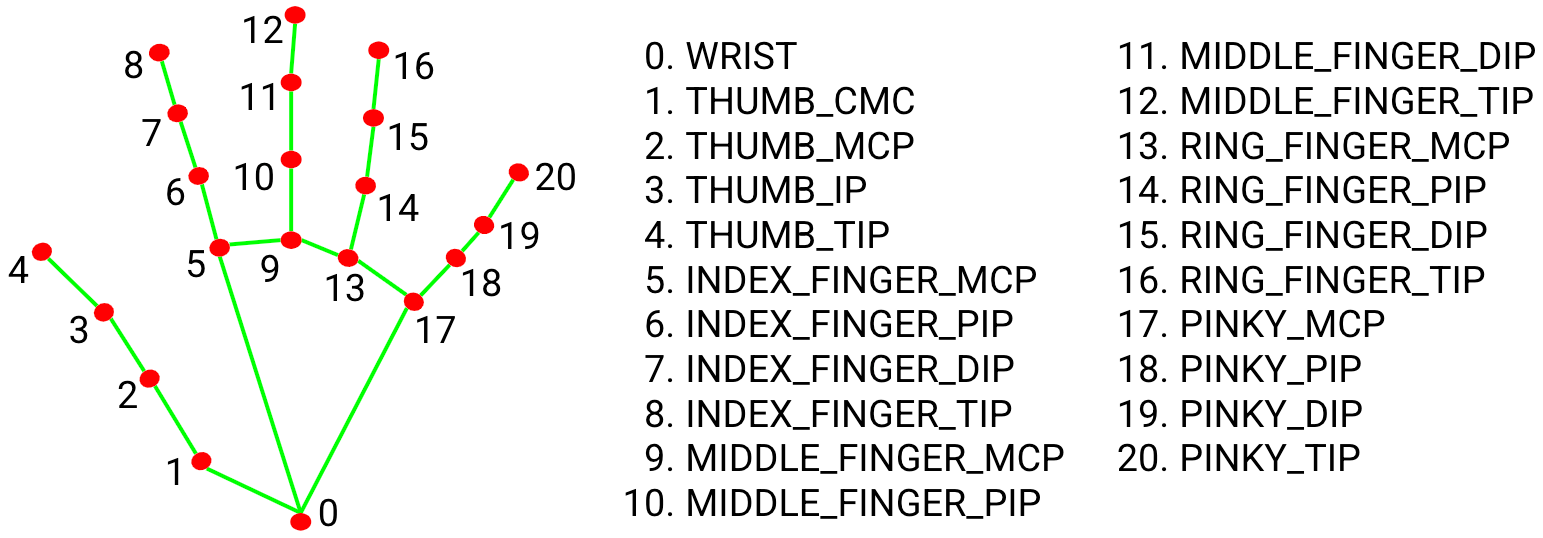
\includegraphics[width=0.9\textwidth]{puntos_mano}
	\centering
	\caption[Puntos de la mano y su nombre.]{Puntos de la mano y su nombre~\cite{mediapipehands}.}
	\label{fig:puntosmano}
\end{figure}

Una vez establecidos los puntos, se van a obtener las coordenadas de cada fotograma donde están ambos puntos, con el fin de obtener la distancia que los separa en cada instante.

\section{Limpieza de los datos}
Dado que la obtención de los datos del paso anterior no es perfecta, hay que utilizar alguna técnica para eliminar el posible ruido que la biblioteca ha podido ocasionar. Este ruido viene dado porque entre fotogramas, la biblioteca puede detectar el dedo en lugares diferentes sin que este se haya movido, provocando que la amplitud de la pinza se vea afectada.

\subsection{Filtro de Savitzky–Golay}
Este filtrado~\cite{wiki:savgol} ha sido utilizado para eliminar algunas imperfecciones de los datos. Se basa en el cálculo de una regresión polinomial local de grado $k$ con al menos $k+1$ puntos equiespaciados que determinan el valor de un nuevo punto. Esto hará que los datos varíen y se suavice la gráfica. 

Al dibujar los datos en forma de gráfica, como se observa en la figura \ref{fig:graficadistancias}, se puede apreciar cómo algunas zonas no establecen un único máximo o el máximo podría estar exagerado, por lo que es necesario suavizar esos picos para obtener un solo máximo. 

\begin{figure}[h]
	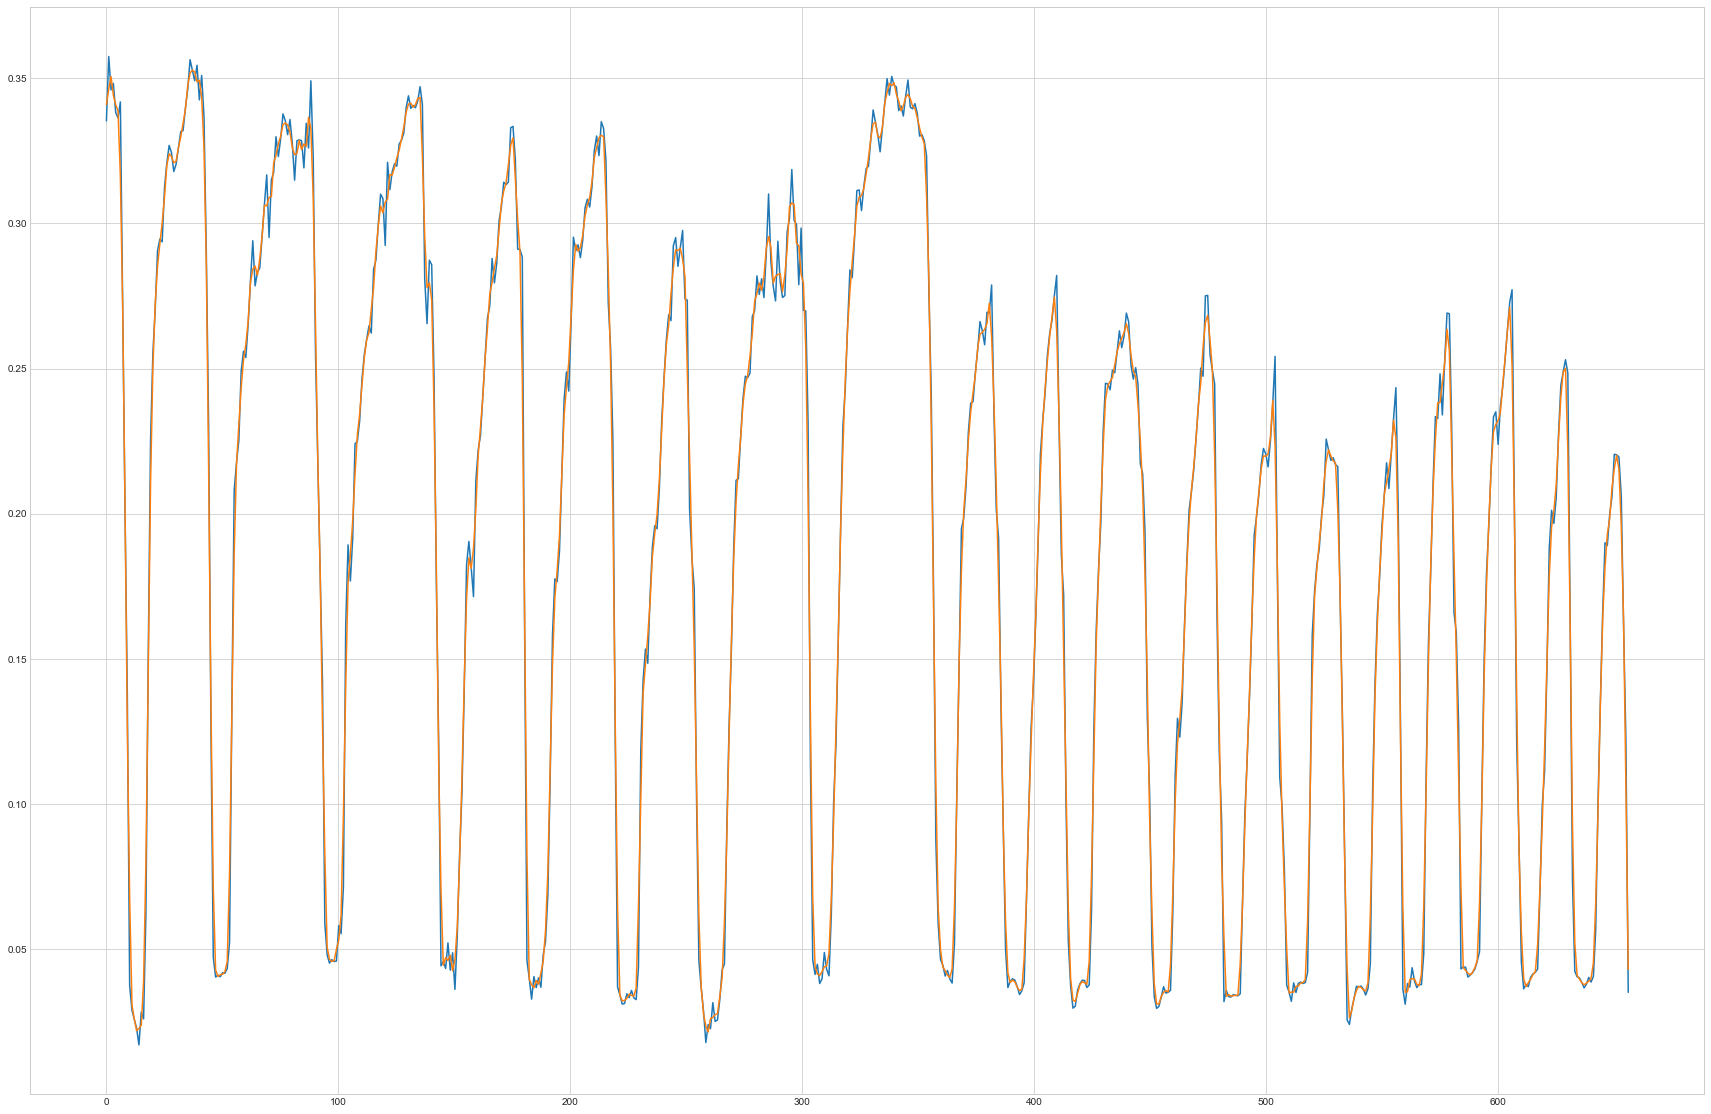
\includegraphics[width=1\textwidth]{grafica_distancias}
	\centering
	\caption[Representación gráfica de los datos obtenidos en uno de los vídeos con y sin filtrado.]{Representación gráfica de los datos obtenidos en uno de los vídeos sin filtrado (azul) y con filtrado (naranja).}
	\label{fig:graficadistancias}
\end{figure}

La figura \ref{fig:graficadistanciaszoom} muestra uno de los picos de forma ampliada, notándose el suavizado del filtro frente a la gráfica sin suavizar eliminando los picos que producen ruido. Lo ideal sería que la curva fuese lo más perfecta posible, pero el propio pulso de la mano y, sobre todo, la biblioteca que coloca los puntos sobre la mano provocan esas imperfecciones que conviene solucionar. No obstante, aun aplicando el filtrado, no se consigue el resultado ideal, pues el filtrado es únicamente aproximación y una mejora del resultado real.

\begin{figure}[h]
	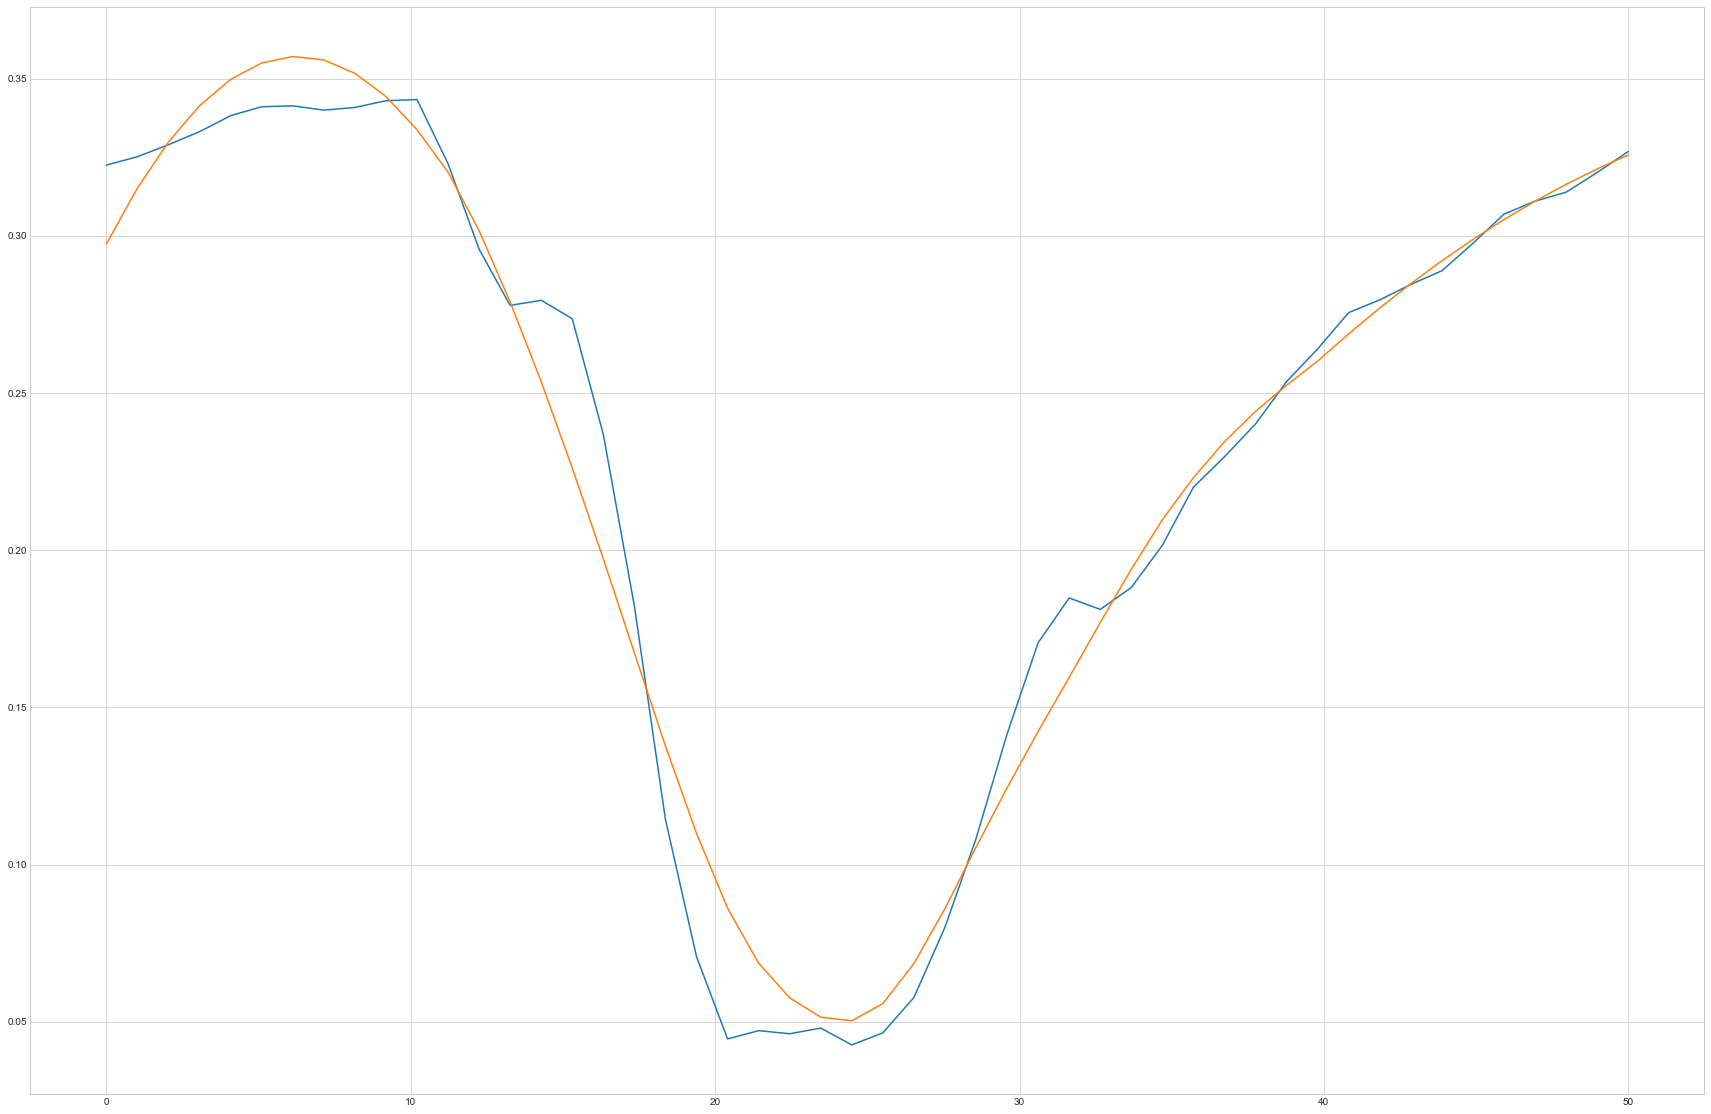
\includegraphics[width=1\textwidth]{grafica_distancias_zoom}
	\caption[Ampliación de uno de los picos donde se aprecia la curva con y sin suavizado.]{Ampliación de uno de los picos donde se aprecia la curva sin suavizar (azul) de la suavizada con el filtro (naranja).}
	\label{fig:graficadistanciaszoom}
\end{figure}

\section{Minería de datos}
Este punto trata de encontrar patrones en los datos que sirvan para clasificar. Para el problema planteado de predicción, hay que utilizar la clasificación.

La clasificación es una tarea de la minería de datos que realiza un proceso de asignación de una clase u otra dependiendo de los valores que tengan los datos. Extrapolado a este trabajo, esto sería asignar si una persona tiene Parkinson o no dependiendo de las características obtenidas en el punto anterior.

\subsection{Conjunto de ejemplos}
Las características obtenidas son las que conforman el conjunto de datos. Este conjunto de datos será mejor cuantos más ejemplos haya, ya que más opciones podrán abarcar los clasificadores y mejores serán las predicciones.

Los clasificadores se utilizan realizando una separación del conjunto total de los datos. Esta separación da lugar a los datos de entrenamiento y los datos de test:

\begin{itemize}
	\item Conjunto de entrenamiento: constituye la mayor parte de los datos, entre el 70 \% y 80 \% generalmente. Sirve para enseñar al modelo a clasificar el conjunto de datos, indicándole qué casos son de una clase y que casos de otra.
	\item Conjunto de test: Sirve para probar cuánto de bueno es el modelo entrenado con los ejemplos de entrenamiento. Tras las predicciones, se comprobará la clase asignada a cada ejemplo y la clase real y se obtendrán unas precisiones.
\end{itemize}

El conjunto de entrenamiento ha de contener más ejemplos que el conjunto de test debido a que cuanto más ejemplos se ofrezcan al modelo, más probable es que aprenda correctamente. Además, para probar cómo de bueno es un modelo, no son necesarios un alto número de ejemplos.

Es importante que a la hora de evaluar el modelo se utilicen datos que no han sido utilizados para entrenar el modelo, ya que esos ejemplos siempre los acertarían. Debido a esto, es necesario tener estas dos divisiones.

\subsection{Validación cruzada}
La validación cruzada es una técnica que se utiliza a la hora de entrenar y probar modelos de aprendizaje. Se basa en dividir el conjunto de datos en un número de partes y utilizar cada una de las partes como conjunto de test y el resto para entrenar el modelo, tal y como se aprecia en la figura \ref{fig:valcruzada}. Cada una de las partes será utilizada como conjunto de test de forma iterativa.

\begin{figure}[h]
	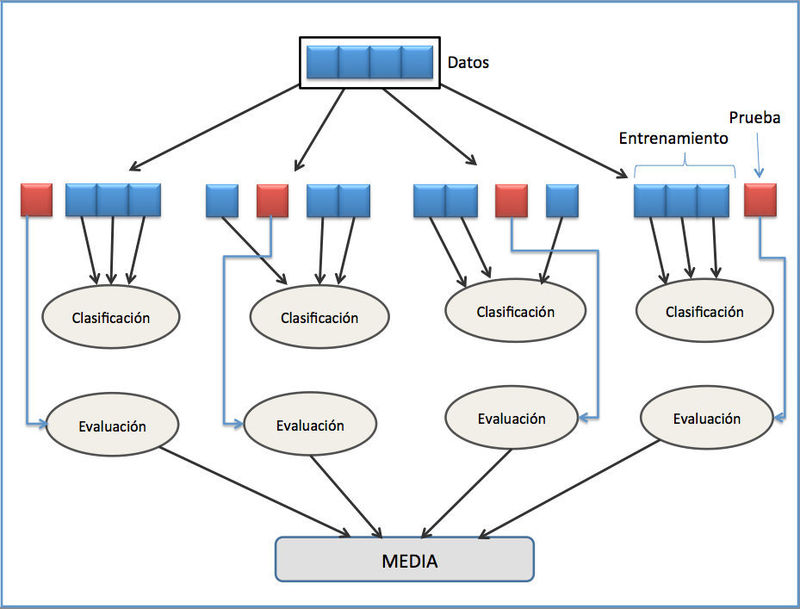
\includegraphics[width=1\textwidth]{validacion_cruzada}
	\caption[Validación cruzada dividendo el conjunto de ejemplos en 4 partes.]{Validación cruzada dividendo el conjunto de ejemplos en 4 partes.\cite{wiki:valcruzada}}
	\label{fig:valcruzada}
\end{figure}

Con esto se consigue que la selección de los conjuntos de entrenamiento y test no perjudique al resultado del modelo y se puedan probar más posibilidades de división de los datos.

\subsection{Modelos de clasificación}
Una de las formas más sencillas de encontrar patrones en los datos es utilizando modelos de aprendizaje. Hay varios modelos, y cada uno utiliza una forma de clasificar diferente. Los modelos empleados en este TFG son:
\begin{itemize}
	\item \textbf{Árboles de decisión:} se trata de construir un árbol formado por nodos con condiciones y hojas con clases, para que los datos sean clasificados dependiendo de si cumplen una condición de un nodo o no.
	\item \textbf{Random Forest:} se trata de clasificar los ejemplos utilizando varios árboles de decisión. Estos árboles se construyen utilizando un subconjunto del conjunto total de datos de entrenamiento. Cada árbol predirá una clase, y la más frecuente será la que se le asigne al atributo.
	\item \textbf{k-Nearest Neighbors:} se trata de obtener la clase de los vecinos más cercanos al ejemplo que se trata de clasificar. En este clasificador, no hay un paso previo de entrenamiento, sino que los datos de entrenamiento serán los que contengan los k vecinos más cercanos.
	\item \textbf{Naive Bayes:} se trata de calcular la frecuencia de aparición de los valores de cada característica para poder realizar una clasificación. Esto haría que 
	un ejemplo con ciertos valores se le asigne una clase debido a la probabilidad de aparición de sus valores.
	\item \textbf{Naive Bayes Gaussiano:} es una variante del clasificador Naive Bayes y se trata de utilizar las probabilidades de que aparezcan los valores de, pero acorde con una distribución normal.
	\item \textbf{SVM:} se trata de conseguir un hiperplano que separe los ejemplos que compartan la misma clase del resto. A la hora de clasificar un ejemplo, dependiendo de dónde se encuentre, se le asignará una clase u otra.
\end{itemize}

\section{Evaluación de los resultados}
A la hora de evaluar los resultados, es importante realizar un estudio de los datos obtenidos para poder valorar correctamente los resultados.

\subsection{Predicciones}
Cuando se utiliza un clasificador, se realizan varias predicciones con el conjunto de test. En esta ocasión, hay dos clases posibles: sin Parkinson (0) o con Parkinson (1), por lo que pueden ocurrir cuatro posibilidades:

\begin{itemize}
	\item Verdadero positivo o \textit{true positive}: ocurre cuando una clase se predice correctamente y además es positiva. En este caso, sería que el clasificador ha predicho un 1 (positivo) y ha acertado. Suele indicarse como TP.
	\item Verdadero negativo o \textit{true negative}: ocurre cuando una clase se predice correctamente y además es negativa. En este caso, sería que el clasificador ha predicho un 0 (negativo) y ha acertado. Suele indicarse como TN.
	\item Falso positivo o \textit{false positive}: ocurre cuando una clase no se predice correctamente y además es positiva. En este caso, sería que el clasificador ha predicho un 1 (positivo) y ha fallado. Suele indicarse como FP.
	\item Falso negativo o \textit{false negative}: ocurre cuando una clase no se predice correctamente y además es negativa. En este caso, sería que el clasificador ha predicho un 0 (negativo) y ha fallado. Suele indicarse como FN.
	
\end{itemize}

\subsection{Medidas}
Las medidas son formas de representar los resultados para obtener diferentes puntos de vista a la hora de evaluar los resultados. Las medidas utilizadas en este TFG son:

\begin{itemize}
	\item \textit{accuracy}: con esta medida se podrá obtener la precisión que ha tenido el clasificador. Esto es, el porcentaje de aciertos que ha habido. La fórmula que se utiliza es la siguiente:
	\begin{equation}
		accuracy = \frac{TP + TN}{TP + TN + FP + FN}
	\end{equation}

	\item \textit{Matthews correlation coefficient}: esta mediada es utilizada para conocer la calidad de una clasificación binaria. La fórmula para obtener esta medida es la siguiente:
	\begin{equation}
		MCC = \frac{TP\times TN-FP\times FN}{\sqrt{(TP+FP)\times(TP+FN)\times(TN+FP)\times(TN+FN)}}
	\end{equation}

	\item \textit{f1}: esta medida es utilizada para recoger las medidas de \textit{precision} y \textit{recall} en una sola medida. La medida \textit{precision} sirve para conocer los aciertos que ha habido en una clase concreta y la medida \textit{recall} sirve para conocer cuántos ejemplos han sido clasificados como una clase concreta. Estas fórmulas son las siguientes:
	\begin{align}
		precision &= \frac{TP}{TP+FP} &
		recall &= \frac{TP}{TP+FN}
	\end{align}
	
	Y la fórmula para obtener la medida f1 es la siguiente:
	\begin{equation}
		f1 = 2\times \frac{precision\times recall}{precision + recall}
	\end{equation}

	\item \textit{roc\_auc}: esta medida es el área bajo la curva ROC y representa cómo de bueno es un modelo a la hora de diferenciar una clase de otra. Dado que esta métrica es más complicada que las anteriores, más abajo se explica de forma más detallada.
	\item \textit{g\_mean}: esta medida es la media geométrica de la sensibilidad y la especificidad y trata de mostrar la precisión de las clases manteniendo las precisiones de forma equilibrada. Las fórmulas de sensibilidad y especificidad, se pueden ver más abajo. La fórmula para obtener esta medida es la siguiente:
	\begin{equation}
		g\_mean = \sqrt{sensibilidad \times especificidad}
	\end{equation}
\end{itemize}

\subsection{Curva ROC}
La curva ROC~\cite{wiki:roc} (\textit{Receiver Operating Characteristic}) es una representación gráfica utilizada para conocer la proporción de positivos bien clasificados y los positivos mal clasificados.

La curva ROC representada gráficamente tiene como eje $x$ la 1-especificidad y como eje $y$ la sensibilidad. La especificidad corresponde a los ejemplos negativos bien clasificados, o lo que es lo mismo, 1 menos los ejemplos positivos mal clasificados; y la sensibilidad corresponde a los ejemplos positivos bien clasificados. Sus correspondientes fórmulas son las siguientes:

\begin{align}
	especificidad &= \frac{TN}{FP+TN} &
	sensibilidad &= \frac{TP}{TP+FN}
\end{align}

Para dibujar la curva ROC habría que recoger varios resultados de un modelo y unir esos puntos para formar la curva, de forma que quede de forma similar que en la figura \ref{fig:roc}, en donde se visualizan tres tipos de curvas ROC que representan clasificaciones de mejor a peor.

\begin{figure}[h]
	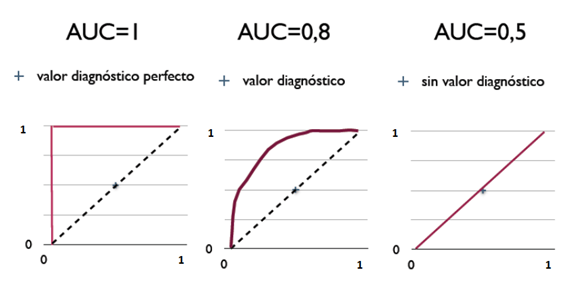
\includegraphics[width=1\textwidth]{curvas_roc}
	\caption[Tres tipos de curvas ROC.]{Tres tipos de curvas ROC~\cite{wiki:roc}.}
	\label{fig:roc}
\end{figure}

\subsection{Área bajo la curva ROC}
El área bajo la curva ROC (\textit{Area Under the ROC Curve}) es la medida con la que conocer cómo de bien un modelo diferencia una clase de otra.

Este área no es más que el cálculo de todo el área que hay debajo de la curva ROC. Los valores obtenidos estarán en el intervalo [0,1]. Los valores comprendidos entre 0 y 0.5 indican que el modelo confunde una clase con otra en su mayor parte, mientras que los valores comprendidos entre 0.5 y 1 indican que el modelo predice correctamente la mayoría de ejemplos, siendo el valor 1 la perfección. En la figura \ref{fig:roc} se aprecian tres valores AUC para cada curva, mostrando que la primera trata de un clasificador perfecto mientras que la última muestra un clasificador mucho peor.

		\capitulo{4}{Técnicas y herramientas}
\section{Herramientas de desarrollo}
\subsection{Anaconda}
Anaconda es una distribución libre utilizada para los lenguajes de programación Python y R con el objetivo de realizar aprendizaje automático y ciencia de datos. Entre sus paquetes se encuentra Jupyter Notebook.

\subsection{Jupyter Notebook}
Jupyter Notebook es un entorno de programación para Python basado en la web. Se pueden crear varios notebooks con celdas de código o texto para conseguir una estructura limpia y ordenada. Además, estos notebooks pueden ser usados para otros lenguajes de programación como Julia o R.

\subsection{Flask}
Flask es un framework que utiliza Python utilizado para crear aplicaciones web. Ofrece sencillez a la hora de programar ya que cuenta con un motor de plantillas que ofrecen la posibilidad de realizar código HTML dinámico.

\subsection{Visual Studio Code}
Visual Studio Code es un entorno de programación con una amplia variedad de elementos que ayudan a programar. Se puede cargar una carpeta entera y poder ver su contenido en forma de árbol para agilizar el acceso a los ficheros de un proyecto.

\subsection{TeXstudio}
TeXstudio es un entorno para crear documentos utilizando el lenguaje \LaTeX{}. En él se pueden utilizar los comandos de \LaTeX{}, además de compilar el código y generar el documento PDF.

\subsection{XAMPP}
XAMPP es un programa que funciona como gestor de bases de datos MySQL y servidores Apache. Además, puede contener otras aplicaciones compatibles con Apache. En este trabajo el servidor de Apache no es utilizado, ya que se utiliza el servidor de Flask, pero es necesario para la base de datos MySQL.

\subsection{Bootstrap}
Bootstrap es una biblioteca de código abierto desarrollada por Twitter que se utiliza para realizar diseños de páginas web. Cuenta con muchos diseños de botones, menús, barras de navegación, formularios, iconos, etc. Cuenta con código HTML, CSS y JavaScript para establecer los diseños.

\subsection{draw.io}
draw.io es un software utilizado para realizar diagramas de flujo, diagramas UML, organigramas, entre otros, con posibilidad de guardarlo en la nube. Contiene una plantilla y diversos bloques para realizar los dibujos.

\subsection{GitHub}
GitHub es utilizado para realizar control de versiones en gestión de proyectos ágiles. Se puede subir documentos y código sobre el proyecto, asignar tareas, realizar la metodología \textit{Scrum}, entre otros. Este TFG estará alojado en GitHub, así como las tareas asignadas en cada \textit{sprint} de \textit{Scrum}.

\subsection{Pencil}
Pencil es un programa utilizado para diseñar interfaces mediante dibujo con bloques. Se pueden dibujar gran variedad de pantallas, como aplicaciones de móvil, programas de ordenador o páginas web.

\section{Bibliotecas}
\subsection{OpenCV}
Es una biblioteca de Python utilizada para visión artificial y es considerada la más popular. Tiene diversos usos, entre ellos destacan el reconocimiento de objetos y la detección de movimiento.~\cite{wiki:opencv}

\subsection{Numpy}
Es una biblioteca de Python utilizada para realizar operaciones matemáticas. También se usa para crear vectores y matrices grandes multidimensionales.~\cite{wiki:numpy}

\subsection{Pandas}
Es una biblioteca de Python utilizada para el análisis de datos. Mediante \textit{dataframes} se pueden recoger datos de hojas de cálculo o bases de datos, almacenarlos para ser tratados en el código y después guardarlos de nuevo.~\cite{wiki:pandas}

\subsection{Mediapipe}\label{lib:mediapipe}
Es una biblioteca de Pyhton utilizada para visión artificial. Una de las funcionalidades que tiene es la de reconocer y enumerar con puntos una mano. La biblioteca procesa una imagen, que podría ser el fotograma de un vídeo, y detecta las manos en ella. Tras detectar las manos, identificará la posición de los dedos mediante coordenadas para poder enumerarlos. Tras esto, los puntos se conectan siguiendo unas reglas, con el fin de poder dibujar la silueta de la mano.
\begin{itemize}
	\item \textit{solutions.hands}: este paquete realiza el reconocimiento de la mano para asignar unos puntos. Hay 21 puntos repartidos por toda la mano, los más interesantes para este proyecto son el 4 (dedo pulgar) y el 8 (dedo índice). Todos los puntos vienen dados con coordenadas $x$, $y$ y $z$. Para acceder a un punto, únicamente será necesario acceder a su posición dentro de la estructura de datos que contiene todos los puntos. \cite{mediapipehands}
	\item \textit{solutions.drawing\_utils}: este paquete es el que se encarga de dibujar los puntos y las conexiones entre ellos sobre la mano.
\end{itemize}

\subsection{SciPy}
Es una biblioteca de Python utilizada para realizar tareas de ciencia e ingeniería como optimización, álgebra lineal, interpolación o procesamiento de señales.~\cite{wiki:scipy}
\begin{itemize}
	\item \textit{signal}: es el módulo que sirve para realizar procesados de señales como convolución o filtrado, entre otros.~\cite{scipysignal}
\end{itemize}

\subsection{Matplotlib}
Es una biblioteca de Python utilizada para realizar representaciones gráficas a partir de conjuntos de datos.
\begin{itemize}
	\item \textit{pyplot}: este módulo es utilizado para mostrar gráficos como figuras con el fin de poder configurar, entre más opciones, su tamaño. \cite{plt}
\end{itemize}

\subsection{Imbalanced learn}
Es una biblioteca de Python utilizada para realizar aprendizaje automático con conjuntos que no se encuentran equilibrados.
\begin{itemize}
	\item \textit{metrics}: este módulo contiene las métricas utilizadas en aprendizaje automático, pero teniendo en cuenta conjuntos de datos desequilibrados. \cite{imblearn}
\end{itemize}

\subsection{Scikit-learn}
Es una biblioteca de Python utilizada para realizar aprendizaje automático. Se pueden entrenar modelos de aprendizaje, tanto de regresión como de clasificación, entre otras posibilidades.
\begin{itemize}
	\item \textit{ensemble}: este módulo contiene varios ensembles con los que realizar predicciones. \cite{skensemble}
	\item \textit{metrics}: este módulo contiene un gran número de métricas utilizadas en aprendizaje automático. \cite{skmetrics}
	\item \textit{model\_selection}: este módulo contiene todos aquellos métodos encargados de realizar selección de datos, como la validación cruzada. \cite{skmodsel}
	\item \textit{naive\_bayes}: este módulo contiene algoritmos de aprendizaje supervisado basados en el teorema de Naive Bayes. \cite{sknbayes}
	\item \textit{neighbors}: este módulo contiene los algoritmos de aprendizaje basados en los vecinos más cercanos. \cite{skneighbors}
	\item \textit{tree}: este módulo contiene los clasificadores basados en árboles de decisión. \cite{sktree}
	\item \textit{dummy}: este módulo contiene los predictores de clasificación y regresión más sencillos.
	\item \textit{svm}: este módulo contiene los predictores basados en máquinas de soporte vectorial. \cite{sksvm}
\end{itemize}

\subsection{Joblib}
Es una biblioteca de Python utilizada para almacenamiento en disco. Una de las funcionalidades es la de serializar objetos para almacenarlos en disco y después deserializarlos en otro archivo para poder utilizarlos. Estos archivos tienen la extensión \textit{.pkl}, que es un archivo de Python binario. Permite realizar la serialización de forma rápida y sencilla.

		\capitulo{5}{Aspectos relevantes del desarrollo del proyecto}
En este apartado, se detallan los aspectos más relevantes que han ocurrido durante el desarrollo del proyecto, así como la manera en la que el proyecto ha sido realizado para cumplir los objetivos propuestos.

\section{Limpieza de datos}
Como ya se ha explicado en el punto \ref{limpieza}, los datos obtenidos pueden contener ruido que perjudique la tarea que se quiere realizar, en este caso, la clasificación. Por esta razón, es necesario corregirlos de alguna manera.

\subsection{Filtro de Savitzky-Golay}
En el apartado de conceptos teóricos \ref{savgol}, ya se mencionó el filtro de Savitzky-Golay, con el que se podían mejorar las gráficas representando los resultados obtenidos.

Estos resultados contienen ruido tanto por el propio pulso de la mano como por la biblioteca que detecta la mano, por lo que su representación en ocasiones muestra demasiados máximos o mínimos parecidos, confundiendo los valores reales.

\subsection{Distancias} 
Las distancias ya obtenidas no muestran la distancia  real, por lo que es necesario realizar un paso previo antes de calcular el resto de características que dependen de la distancia. 

Dado que la pinza cerrada es el momento en el que menos distancia hay, lo lógico sería pensar que esta distancia es 0, sin embargo, esto no ocurre debido a la localización de los puntos de los dedos. Estos puntos no están justo en la yema de los dedos, donde la pinza se cierra, sino que están en el centro del dedo, por lo que la distancia entre esos puntos nunca será 0, aunque sí muy próxima, es decir, las distancias mínimas nunca serán 0. Al igual que sucede con las distancias mínimas, también las distancias máximas se ven afectadas, y en general, todas las distancias. Por esta razón, se realizan nuevamente las restas de los máximos y mínimos de las distancias anteriormente calculadas para que los nuevos mínimos alcancen valores mucho más cercanos al 0. 

Para comprender esto mejor, se va a suponer que una distancia mínima entre los dos dedos es de 0,051 y una distancia máxima es de 0,376. Al igual que el 0,051 no es el mínimo real, pues lo lógico sería que fuese 0, la verdadera amplitud máxima tampoco sería real, pues debería contar desde el 0. Para obtener la distancia real habría que obtener la diferencia entre el máximo y el mínimo, para conocer la distancia que les separa, es decir, la amplitud de la pinza, que sería 0,325. 

Realmente, todos los puntos no están recogiendo valores reales, sin embargo, dado que sólo interesa recoger la distancia máxima, únicamente se realiza la diferencia entre máximos y mínimos.

\section{Obtención de características}
En este punto se trata de buscar otros datos que caractericen a los vídeos con el fin de poder realizar una clasificación. Habrá datos calculados y datos que ya vienen dados porque no se pueden calcular, como la mano, la edad o el sexo.

\subsection{Amplitud}
Esta característica es la más evidente ya que, generalmente, los pacientes con Parkinson ven dificultad a la hora de abrir y cerrar la mano hasta su punto máximo.

Para su extracción, en primer lugar, se han recogido los máximos y mínimos de la gráfica de los 5 primeros movimientos y de los 5 últimos. Después, estos datos se normalizan para que no afecte la distancia de la mano a la cámara. Esta normalización se obtiene de la siguiente fórmula:

\begin{equation}
	X_{normalizada} = \frac{X_{actual} - X_{mínima}}{X_{máxima}-X_{mínima}}
\end{equation}

Para la extracción de las distancias, tanto la original como la normalizada, tan solo hay que restar el mínimo con el máximo correspondiente. 

\subsection{Tiempo}
Otra de las características que podrían afectar a una persona que tiene Parkinson es cuánto tardaría en realizar el movimiento de pinza, ya que, en un principio, aquellos que padezcan la enfermedad tardarán más.

Para ello, se ha realizado la diferencia entre un máximo y el mínimo correspondiente. En este caso se ha utilizado como unidad temporal el número de fotogramas entre ambos puntos, ya que, a más lentitud, más fotogramas habrá de diferencia y viceversa.

Sin embargo, esta medida resulta no ser suficiente porque no se tiene en cuenta cuánto se ha abierto la pinza, es decir, alguien que abra la pinza lentamente y hasta la mitad tardará el mismo tiempo que alguien que la abra más rápido y hasta el máximo.

\subsection{Velocidad}
Para solucionar el problema anterior, se puede utilizar la velocidad. Esto es, calcular la distancia recorrida por unidad de tiempo, por lo que dependiendo de cuánto se recorra y en cuánto tiempo, una persona tendrá más velocidad o no.

En una primera instancia, una persona que padece Parkinson, dada su reducida movilidad, pese a abrir la pinza hasta su punto máximo, lo más seguro es que lo hiciera de forma más lenta que otra persona sin Parkinson.

Esta velocidad se calcula realizando la división de la diferencia normalizada entre un máximo y un mínimo (\textit{i. e.} la amplitud ya calculada), entre el tiempo que les separa a ambos puntos (\textit{i. e.} el tiempo ya calculado).

Para este trabajo, se ha calculado la velocidad media de cada vídeo.

\subsection{Mano derecha o izquierda}
Como añadido, también se ha tenido en cuenta si la mano es derecha o izquierda. En un principio, podría resultar interesante conocer cuál es la mano que más dificultades tiene a la hora de realizar el movimiento, aunque tampoco resulta fundamental para clasificar. Esta característica no es calculada, sino que viene dada con el vídeo.

\subsection{Sexo}
El sexo de la persona podría servir para clasificar las personas con y sin Parkinson. Como se ha mencionado en la introducción de este documento, el Parkinson es más propenso a aparecer en hombres, por lo que, en primera instancia, podría haber más hombres con Parkinson que mujeres, o lo que es lo mismo, más mujeres sin Parkinson que hombres, lo cual podría ayudar a la hora de clasificar. Al igual que con la mano, esta característica no es calculada, sino que viene dada con el vídeo.

\subsection{Edad}
De forma similar a lo que ocurre con el sexo, el Parkinson es más propenso en personas mayores, de 60 años, por lo que la edad también podría resultar interesante a la hora de clasificar.

Sin embargo, hay que tener cuidado con los ejemplos a la hora de entrenar modelos, ya que el sistema podría aprender que todos los menores de, por ejemplo, 30 años nunca tendrán Parkinson, cuando esto no es cierto. Esto dependerá de la muestra de entrenamiento, ya que si hay pacientes de diversas edades con Parkinson, el modelo realizará la predicción teniendo en cuenta también esos casos. 

Pese a poder ser interesante, esta característica con los datos utilizados no mejora los resultados, por lo que finalmente no será utilizada. Esta característica tampoco es calculada, también viene dada con el vídeo.

\section{Resultados} \label{resultados}
Para obtener mejores resultados es importante que el conjunto de datos utilizado para entrenar el modelo esté equilibrado. Sin embargo, estos resultados no son tan buenos como se podría esperar, aunque sí se obtiene una diferencia entre aquellos con y sin Parkinson. Este conjunto de datos debería contar con más ejemplos para que el clasificador fuese capaz de distinguir diferentes niveles de Parkinson entre dos pacientes.

Para conocer cuál es el clasificador que mejor predice, se ha realizado un estudio de los resultados, utilizando las métricas ya explicadas en el apartado \ref{medidas}. Además, también se ha realizado un estudio de tiempos, para conocer cuál es el clasificador más rápido.

\subsection{Predicción}
Para realizar la predicción, se han utilizado los clasificadores ya explicados en el apartado \ref{clasificadores}, donde cada columna se corresponde a las siglas de cada clasificador. Se han descartado algunas de las características obtenidas como las amplitudes sin normalizar, la edad o el tiempo ya que empeoraban la clasificación. Además, se ha utilizado una validación cruzada de 2 divisiones y 5 repeticiones, obteniéndose los siguientes resultados:

\begin{table}[h]
	\begin{center}
		\begin{tabular}{ l c c c c c c c }
			\toprule
			\textbf{Medidas} & \textbf{RF} & \textbf{k-NN} & \textbf{AD} & \textbf{NBG} & \textbf{SVM} & \textbf{NB} & \textbf{Dummy} \\ \midrule
			accuracy & 0,719 & 0,544 & 0,669& 0,4888 & 0,562 & 0,575 & 0,562 \\
			Matt. corr. coeff. & 0,435 & 0,084 & 0,315 & -0,015 & 0,013 & 0,075 & 0 \\ 
			f1 & 0,75 & 0,577 & 0,71 & 0,482 & 0,707 & 0,708 & 0,72 \\
			ROC AUC & 0,776 & 0,547 & 0,663& 0,467 & 0,57 & 0,521 & 0,5 \\
			g mean & 0,706 & 0,522 & 0,609 & 0,468 & 0,056 & 0,252 & 0 \\ \bottomrule
		\end{tabular}
		\caption{Tabla con las medidas y clasificadores utilizados.}
		\label{tab:medidas}
	\end{center}
\end{table}

Lo más destacable de estos resultados es el área bajo la curva ROC (\textit{ROC AUC}) y la precisión (\textit{accuracy}), siendo el clasificador Random Forest el mejor en ambos.

El área bajo la curva ROC del clasificador es 0,776, y significa que gran parte de los ejemplos los diferencia correctamente, sin confundir una clase con la otra. En general todos los clasificadores realizan una clasificación bastante decente, ya que diferencian más o menos bien los ejemplos de una clase de los de la otra, a excepción del clasificador Naive Bayes Gaussiano. Si este clasificador se utilizara a la inversa, esto es, cuando prediga sí decir no y viceversa, tendría un valor de 0,533 ($1 - 0,467$), que aunque no sea demasiado optimista, sería mejor que utilizarlo tal y como está.

Por otro lado, la precisión indica que hay un 71,9 \% de ejemplos bien clasificados, teniendo en cuenta que además los está identificando bien. 

\subsection{Tiempos de entrenamiento}
Se ha realizado un estudio de los tiempos que tardan en entrenar los modelos. Para ello, se han realizado 10 ejecuciones con cada modelo para conocer una aproximación del tiempo que tardan en entrenar, donde se han obtenido los siguientes resultados en segundos:

\begin{table}[h]
	\begin{center}
		\begin{tabular}{ l c c c c c c c }
			\toprule
			\textbf{Ejecuciones} & \textbf{RF} & \textbf{k-NN} & \textbf{AD} & \textbf{NBG} & \textbf{SVM} & \textbf{NB} & \textbf{Dummy} \\ \midrule
			1 & 0,32934 & 0,00397 & 0,00347 & 0,00294 & 0,005 & 0,00505 & 0,00046 \\
			2 & 0,33381 & 0,00391 & 0,00297 & 0,00347 & 0,00561 & 0,00449 & 0 \\ 
			3 & 0,28417 & 0,00319 & 0,00198 & 0,00347 & 0,00546 & 0,00496 & 0,0006 \\
			4 & 0,32095 & 0,00362 & 0,00347 & 0,00347 & 0,00493 & 0,00534 & 0 \\
			5 & 0,26536 & 0,00248 & 0,00198 & 0,00542 & 0,00592 & 0,00496 & 0,0005 \\
			6 & 0,32885 & 0,00149 & 0,00294 & 0,00347 & 0,00545 & 0,00465 & 0 \\
			7 & 0,33331 & 0,00248 & 0,00397 & 0,00298 & 0,00552 & 0,00493 & 0,0005 \\
			8 & 0,32438 & 0,00248 & 0,00298 & 0,00397 & 0,00397 & 0,00496 & 0 \\
			9 & 0,245 & 0,00199 & 0,00252 & 0,00446 & 0,00455 & 0,00298 & 0,0005 \\
			10 & 0,28023 & 0,00244 & 0,00296 & 0,00447 & 0,00528 & 0,00308 & 0,0005 \\ \midrule
			Media & 0,30454 & 0,0028 & 0,00292 & 0,00381 & 0,00517 & 0,00454 & 0,00031 \\ \bottomrule
		\end{tabular}
		\caption{Tabla con los tiempos de entrenamiento de cada modelo con las 10 ejecuciones.}
		\label{tab:tiempos_entrenamiento}
	\end{center}
\end{table}

Además, se muestran estos datos en formato de gráfica en la figura \ref{fig:grafico_entrenamiento}.

\begin{figure}[ht]
	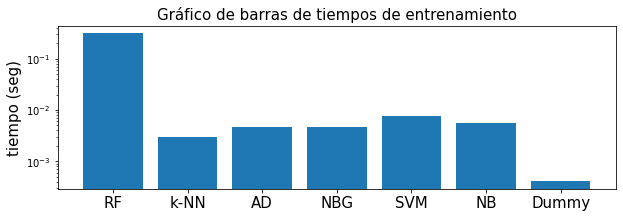
\includegraphics[width=1\textwidth]{grafico_entrenamiento}
	\caption{Gráfico de barras con los tiempos medios de entrenamiento de cada modelo.}
	\label{fig:grafico_entrenamiento}
\end{figure} 

Viendo los resultados, se puede observar que el clasificador que más destaca frente al resto es el Random Forest. Esto se debe a cómo se construye el clasificador. Dado que Random Forest es un \textit{ensemble}, es decir, que está formado por varios clasificadores, en este caso, árboles de decisión, tiene que realizar la construcción de cada árbol de decisión para construir el clasificador completo. 

En la otra parte está el clasificador Dummy. Como ya se ha comentado, este clasificador realiza una predicción de la clase mayoritaria, es decir, no necesita tomar decisiones internas sobre qué clase asignar a la instancia que se está clasificando, por lo que no requiere apenas tiempo para construir el clasificador.

\subsection{Tiempos de predicción}
También se ha realizado un estudio de los tiempos que tardan en predecir los modelos. Al igual que sucedía con el estudio anterior, se han realizado 10 ejecuciones con cada modelo para conocer una aproximación del tiempo que tardan en predecir, donde se han obtenido los siguientes resultados:

\begin{table}[h]
	\begin{center}
		\begin{tabular}{ l c c c c c c c }
			\hline
			\textbf{Ejecuciones} & \textbf{RF} & \textbf{k-NN} & \textbf{AD} & \textbf{NBG} & \textbf{SVM} & \textbf{NB} & \textbf{Dummy} \\ \hline
			1 & 0,02381 & 0,00502 & 0,00149 & 0,00301 & 0,00397 & 0,00285 & 0,00053 \\
			2 & 0,03476 & 0,00524 & 0,00099 & 0,00244 & 0,00328 & 0,00347 & 0,00099 \\ 
			3 & 0,01885 & 0,00496 & 0,00251 & 0,00347 & 0,00351 & 0,00344 & 0,00035 \\
			4 & 0,02328 & 0,00333 & 0,00249 & 0,00302 & 0,00405 & 0,00313 & 0,0005 \\
			5 & 0,02083 & 0,00248 & 0,00199 & 0,00347 & 0,00343 & 0,00343 & 0,0005 \\
			6 & 0,03274 & 0,00198 & 0,00149 & 0,00248 & 0,00397 & 0,00332 & 0,0005 \\
			7 & 0,03026 & 0,00397 & 0,00198 & 0,00248 & 0,00341 & 0,00347 & 0,0005 \\
			8 & 0,01891 & 0,00347 & 0,00198 & 0,00347 & 0,00298 & 0.00248 & 0,0005 \\
			9 & 0,02527 & 0,00351 & 0,00198 & 0,00297 & 0,00338 & 0,00198 & 0,0005 \\
			10 & 0,03274 & 0,00347 & 0,0015 & 0,00347 & 0,00368 & 0,00341 & 0,0005 \\ \hline
			Media & 0,02614 & 0,00374 & 0,00184 & 0,00303 & 0,00357 & 0,0031 & 0,00054 \\ \hline
		\end{tabular}
		\caption{Tabla con los tiempos de predicción de cada modelo con las 10 ejecuciones.}
		\label{tab:tiempos_pred}
	\end{center}
\end{table}
 
De nuevo, se muestran estos datos en formato de gráfico en la figura \ref{fig:grafico_prediccion}.
 
\begin{figure}[ht]
 	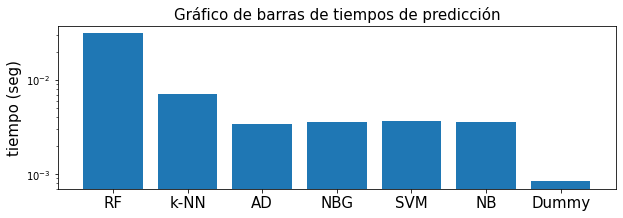
\includegraphics[width=1\textwidth]{grafico_prediccion}
 	\caption{Gráfico de barras con los tiempos medios de predicción de cada modelo.}
 	\label{fig:grafico_prediccion}
\end{figure}
 
 Nuevamente, el clasificador Random Forest lidera la tabla de tiempos, con mucha diferencia del segundo. Esto se debe por la misma razón que en el entrenamiento, es decir, que se trata de un \textit{ensemble}, pues debe realizar varias predicciones con varios árboles de decisión para poder obtener la mejor. Sin embargo, el tiempo medio es muy inferior al anterior, ya que en general, los clasificadores tardan más en construirse que en realizar la predicción. 
 
 Además, vuelve a destacar el clasificador Dummy, con un tiempo medio muy similar al de entrenamiento. El tiempo que tarda en clasificar es prácticamente insignificante, ya que la única tardanza que tiene es la de asignar a cada instancia la clase mayoritaria.
 
 Sin embargo, estos tiempos son prácticamente insignificantes, ya que el clasificador más lento (\textit{i. e.} el Random Forest) tardaría menos de un segundo en entrenar y predecir utilizando este conjunto de ejemplos.
 
 \subsection{Aplicación web}
Uno de los objetivos propuestos en este trabajo es el de realizar una aplicación web para poder predecir si, dado un vídeo de una mano de una persona, esa persona tiene Parkinson o no. Sin embargo, como se ha explicado en puntos anteriores, esta predicción no va a poder ser realizada de la forma ideal, debido a que el conjunto de datos no es demasiado completo como para poder entrenar un clasificador capaz de mostrar una gran diferencia  entre varios niveles de Parkinson. Actualmente, la aplicación predirá entre un 40 y un 50 \% en caso de no tener Parkinson, y entre un 80 y un 90 \% en caso opuesto.

En los resultados de la predicción, se ha destacado el área bajo la curva del clasificador Random Forest, que era superior a la del resto de los clasificadores. Por esta razón, se ha optado por utilizar este clasificador para realizar las predicciones en la aplicación web. No obstante, este modelo puede ser cambiado por el administrador en cualquier momento.

Cualquier vídeo puede ser procesado en la aplicación, siempre y cuando aparezca una mano de forma clara, esta no se salga del vídeo en ningún momento y realice un mínimo de 5 movimientos. Lo ideal para que la aplicación realice la predicción de la forma más rápida y eficaz, sería hacer 10 movimientos, ya que la aplicación escoge los 5 primeros movimientos y los 5 últimos y no tiene en cuenta los movimientos intermedios. Sin embargo, un vídeo con más movimientos podría notar una fatiga en la diferencia entre los 5 primeros movimientos y los 5 últimos, pudiendo afectar en la predicción. Si únicamente se realizan 5 movimientos, la aplicación estaría escogiendo los mismos 5 movimientos ambas veces, y por esta razón, no puede haber menos de 5 movimientos. Además, el número de fotogramas afecta al tiempo de procesado del vídeo, por lo que 5 movimientos realizados de forma lenta tardarán más en procesarse que 5 movimientos realizados de forma más rápida.

Dado que el \textit{software} realizado es una aplicación web, este puede ser utilizado desde dispositivos móviles. Por esta razón, se ha implementado una interfaz diferente para pantallas menores a una anchura, por lo que el menú será más cómodo de utilizar en dispositivos de pantallas pequeñas.

		\capitulo{6}{Trabajos relacionados}
Además de este proyecto, ha habido otros similares en los que se trata de identificar el Parkinson mediante visión artificial con otro tipo de técnicas.

Dada la gravedad de la enfermedad, ha habido varios estudios aplicando diversas formas de detección de Parkinson para facilitar el trabajo de médicos, además de servir a modo de autodiagnóstico.

En este apartado se van a exponer aquellos trabajos que también se dedican a detectar el Parkinson y que están relacionados con este proyecto.

\subsection{A new computer vision-based approach to aid the diagnosis of Parkinson's disease}
Este trabajo~\cite{pereira2016new} consiste en detectar utilizando técnicas de visión artificial si una persona tiene Parkinson o no mediante dibujos de espirales realizados a mano por varias personas.

El primer paso es el de realizar una prueba en la que hay que dibujar las formas tal y como se aprecia en la figura \ref{fig:pruebapapel}, tan solo realizando los ejercicios c y d. En estos ejercicios se trata de realizar la figura de la prueba con un bolígrafo encima de ella sin levantarlo. De esta manera, aquellas personas que padezcan Parkinson quedarán más diferenciadas de las que no, ya que, generalmente, quienes no tengan harán los dibujos más perfectos.

Posteriormente, estos ejercicios son digitalizados para realizar la extracción del dibujo realizado, los cuales se enumeran del 1 al 4 para el ejercicio c y del 5 al 8 para el ejercicio d. Dado que cada individuo realiza 8 dibujos, se acaban obteniendo unos datos. La recogida de datos se realizó tanto a pacientes diagnosticados como a control.

A continuación, el proceso se divide en dos pasos: procesado de imágenes y extracción de características.

El primer paso consiste en separar el dibujo de la persona (HT) del dibujo del papel (ET). Se utilizan técnicas de procesado como filtrado y morfología matemática.

\begin{figure}[ht]
	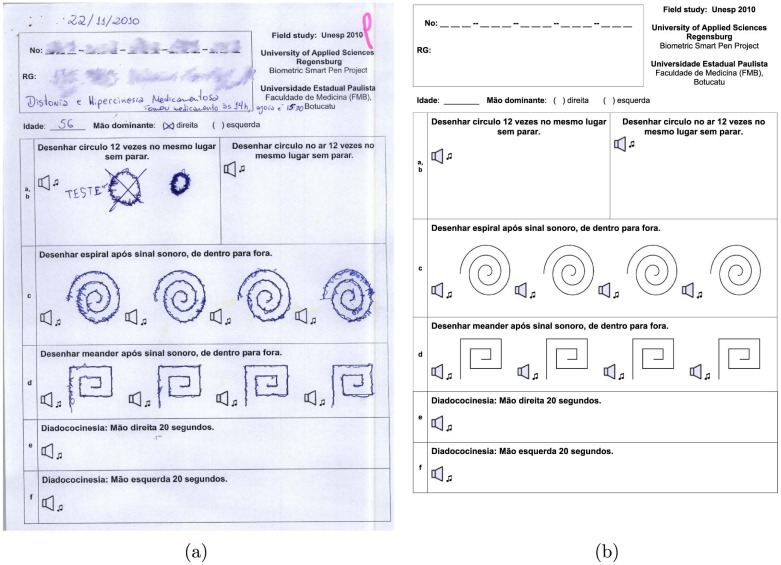
\includegraphics[width=1\textwidth]{prueba_papel}
	\caption[Prueba a papel que realizó una persona con Parkinson en este proyecto y la hoja en blanco de la prueba.]{Prueba a papel que realizó una persona con Parkinson en este proyecto (a) y la hoja en blanco de la prueba (b)~\cite{pereira2016new}.}
	\label{fig:pruebapapel}
\end{figure}

A la hora de obtener el dibujo del paciente (HT), en primer lugar se filtran los dibujos para eliminar el ruido, y en el siguiente paso se utiliza una fórmula que actúe como umbral con el fin de obtener una máscara binaria \(M^{i}_{ET}\ (I)\), tal y como se muestra: 

\begin{equation}
	M^{i}_{ET}\ (I) = \left\lbrace\begin{array}{ll}
0~\text{if}~R^{i}~(I)<100\wedge G^{i}~(I)<100\wedge B^{i}~(I)<100 \\ 1~\text{otherwise,} \end{array}\right.
\end{equation}

\(R^{i}(I)\), \(G^{i}(I)\) y \(B^{i}(I)\) son los valores del espacio de color RGB del píxel \(i\). Una vez obtenida la máscara \(M^{i}_{ET}\ (I)\), se restan los píxeles de la imagen original, obteniendo únicamente el dibujo del paciente.

Por otro lado, se obtiene el dibujo de la prueba (ET) de una manera similar. Se utilizan filtrados para eliminar el ruido y, a continuación, se calcula un umbral mediante una fórmula para obtener una máscara \(M^{i}_{HT}\ (F)\) que en este caso no será binaria, ya que será necesario obtener el color del bolígrafo para poder separarlo y extraer el dibujo del fondo tal y como se muestra:
 
\begin{equation}
	M^{i}_{HT}\ (F) = \left\lbrace\begin{array}{ll}
		255\begin{split}&~\text{if}~|R^{i}~(F)-G^{i}~(F)|<40\wedge |R^{i}~(F)-B^{i}~(F)|<40~\wedge \\ & \wedge|G^{i}-B^{i}|<40 \end{split} \\ F^i~\text{otherwise,} \end{array}\right.
\end{equation}

\(F^{i}\) es la saturación de color del píxel \(i\). Al igual que sucedía en el proceso anterior, cuando se  obtiene la máscara \(M^{i}_{HT}\ (F)\), se restan los píxeles de la imagen original, obteniendo únicamente el dibujo de la prueba.

Finalmente, se obtienen dos imágenes en cada dibujo: el dibujo del paciente y el dibujo de la prueba, como se aprecia en la figura \ref{fig:resultado}.

\begin{figure}[ht]
	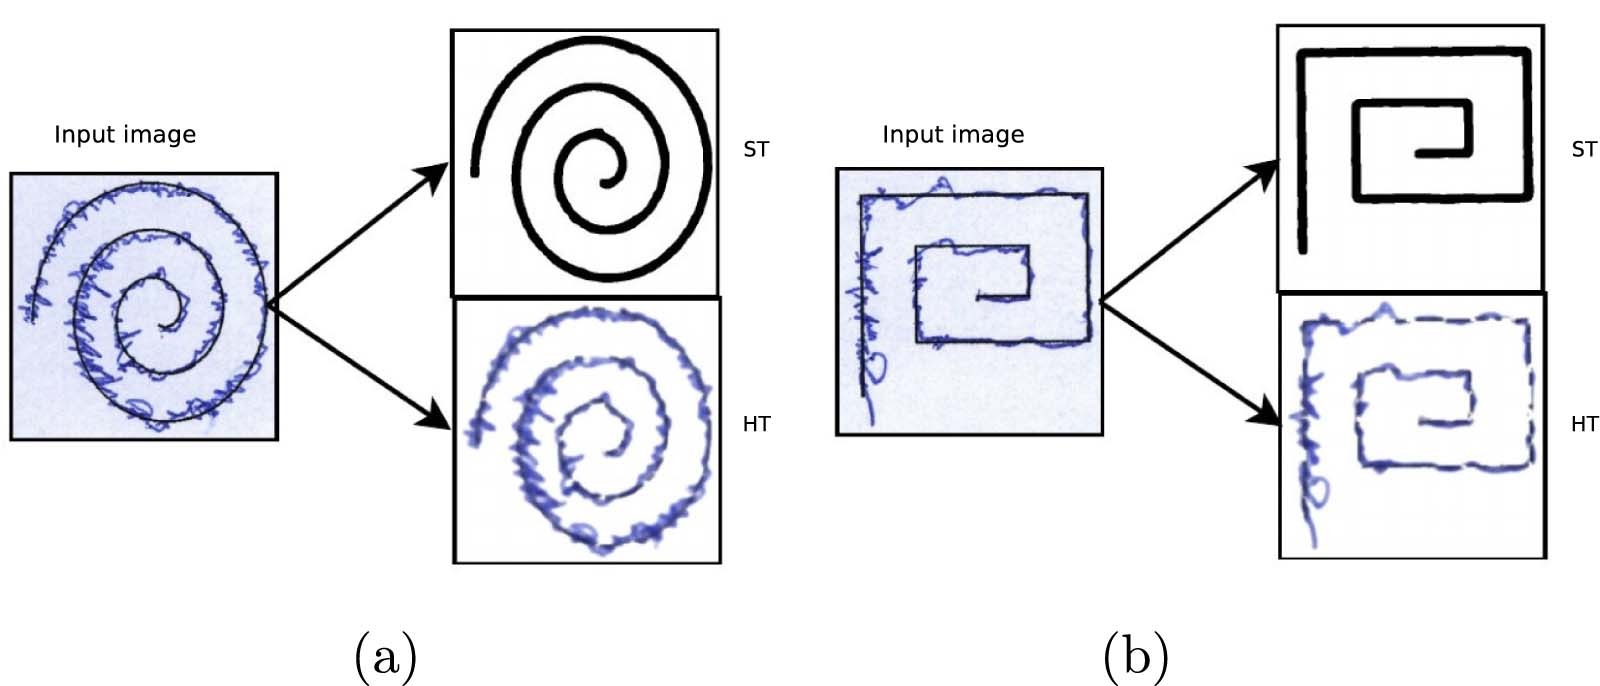
\includegraphics[width=1\textwidth]{resultado_dibujos}
	\caption[Resultado obtenido en cada dibujo de los ejercicios c y d.]{Resultado obtenido en cada dibujo del ejercicio c (a) y del ejercicio d (b)~\cite{pereira2016new}.}
	\label{fig:resultado}
\end{figure}

El segundo paso del proceso consiste en extraer características de los dibujos. Para ello se comparan las dos imágenes obtenidas en el primer paso para evaluar cómo de diferentes son. 

Para facilitar el proceso, se utiliza el algoritmo de adelgazamiento Zhang–Suen~\cite{zhang1984fast}, que resumidamente se encarga de hacer que las trazas de los dibujos aparezcan de forma más fina. Además, se corrigen algunas imperfecciones en las imágenes, como líneas discontinuas. Después, se enumeran algunos puntos en las imágenes y se compara la posición entre dos puntos equivalentes para conocer la desviación del dibujo del paciente con respecto al dibujo de la prueba, obteniendo varios datos con las características de los dibujos. También se obtienen datos obteniendo la distancia entre algunos puntos aleatorios de ambas espirales al centro, ya que la desviación del dibujo del paciente afecta también en su enfermedad de Parkinson. Finalmente, se entrenan los modelos para detectar el Parkinson con todos los datos obtenidos en el paso anterior.

El experimento que se llevó a cabo albergaba dos grupos de personas: uno con gente sin Parkinson y otro con gente con Parkinson. Además, se mezcló en ambos grupos los dos sexos y algún zurdo, frente a una mayoría diestra.

\subsection{Proposing a Three-Stage Model to Quantify
	Bradykinesia on a Symptom Severity Level
	Using Deep Learning}
Este proyecto~\cite{jaber2021proposing} es similar al que se trata en este TFG, ya que también se basa en recoger datos procesando la mano haciendo un movimiento de pinza.

Para ello, se procesan varios vídeos con la mano, tanto izquierda como derecha, habiendo además varios de control. El movimiento realizado debe ser lo más rápido y amplio posible durante 10 segundos.

El preprocesado se realiza utilizando VLC Player para obtener fotogramas de los vídeos. Con Python, y más concretamente, una biblioteca llamada LabelImg se anotan de forma gráfica objetos detectados en la imagen, como se puede observar en la figura \ref{fig:manoetiquetada}.

\begin{figure}[]
	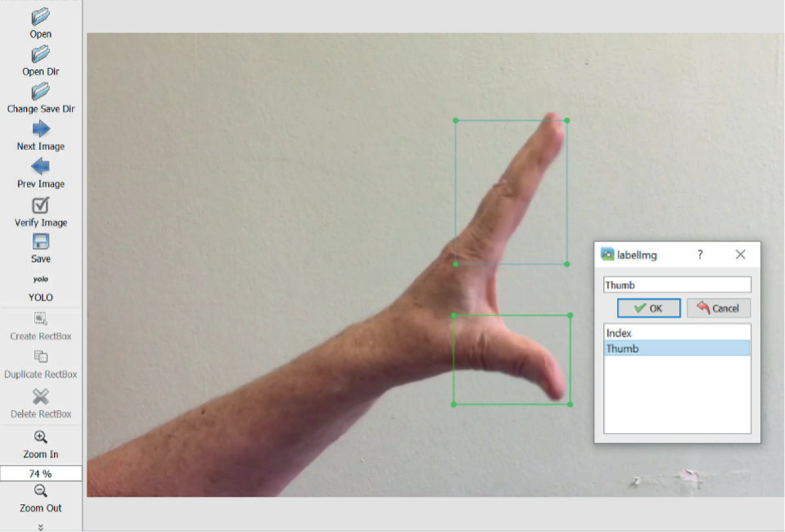
\includegraphics[width=1\textwidth]{mano_etiquetada}
	\caption[Mano con los dedos índice y pulgar etiquetados.]{Mano con los dedos índice y pulgar etiquetados~\cite{jaber2021proposing}.}
	\label{fig:manoetiquetada}
\end{figure}

Eso servirá para recoger las coordenadas de los dedos índice y pulgar y anotarlos en un fichero de texto de la manera:
\begin{center}
	\texttt{< object - class >< x\_center >< y\_center >< width >< height >}
\end{center}

Utilizando la herramienta YOLO, se consigue que los vídeos sean procesados en tiempo real, y así, se obtiene más velocidad en el preprocesado.

Cada recuadro muestra el ID de la clase y la confianza de detección tal y como se ve en la figura \ref{fig:manoetiquetas}. El movimiento se conoce comparando las coordenadas del recuadro con las coordenadas del recuadro que tenía el fotograma anterior, lo cual se almacena para cada fotograma junto al momento en el que se calcula.

\begin{figure}[]
	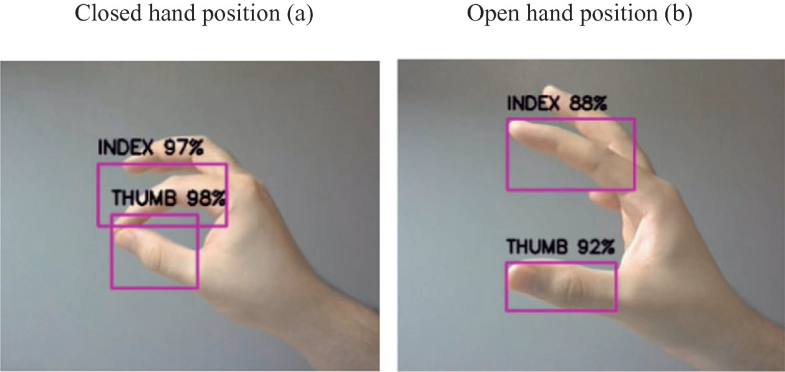
\includegraphics[width=1\textwidth]{mano_etiquetas}
	\caption[Detección realizada con un ajuste ideal.]{Detección realizada con un ajuste ideal~\cite{jaber2021proposing}.}
	\label{fig:manoetiquetas}
\end{figure}

En caso de haber ruido de fondo y/o una orientación de la mano diferente, podría afectar a la confianza de detección, empeorando los resultados obtenidos.

Estos datos obtenidos se utilizan para realizar cálculos con los que sacar conclusiones. Entre los cálculos se encuentran:

\begin{itemize}
	\item Separación: es el desplazamiento entre dos recuadros.
	\item Tiempo: se obtiene extrayendo el fotograma actual y restándole el anterior dividido entre los fotogramas capturados por segundo.
	\item Velocidad: se calcula con la diferencia de separación entre dos fotogramas contiguos dividido entre el tiempo.
	\item Ritmo: es el producto entre la diferencia de separación de dos fotogramas contiguos y su respectiva velocidad.
\end{itemize}

Finalmente, los datos se representan en gráficas observar las diferencias de las personas que padecen Parkinson de las que no y con ello alcanzar conclusiones.

\subsection{The discerning eye of computer vision: Can it measure Parkinson's finger tap bradykinesia?}
En este proyecto~\cite{williams2020discerning}, se ha querido conocer si es posible medir el Parkinson abriendo y cerrando los dedos en forma de pinza, de forma similar a como se hace en el trabajo que representa este documento.

Las mediciones están dentro de la escala MBRS (\textit{Modified Bradykinesia Rating Scale}), que evalúa la velocidad, la amplitud y el ritmo de los movimientos y de la escala MDS-UPDRS~\cite{goetz2008mds} (\textit{Movement Disorder Society revision of the Unified Parkinson's Disease Rating Scale}), que se encarga de evaluar aspectos que tiene el Parkinson con respecto a experiencias motoras y no motoras del día a día.

Como herramienta, se utilizó DeepLabCut, que es una herramienta muy similar a la biblioteca Mediapipe de Python que ya se ha explicado en este documento, en la que cualquier parte del cuerpo es marcada con unos puntos para obtener datos acerca de cómo se está moviendo. Sin embargo, para este proyecto sólo se utilizó la herramienta para las manos.

Los puntos de la mano, se utilizaron para conocer el movimiento de los dedos al realizar el movimiento de pinza, creando coordenadas de los dedos para cada vídeo. Estas coordenadas son las que se utilizaron para obtener la distancia entre los dedos. Además, al igual que en el proyecto que se presenta en el documento, en este también se utilizó el filtrado Savitzky-Golay para eliminar algunos errores que pudiera ocasionar la herramienta.

Los datos que se extrajeron sirvieron para obtener la amplitud, la velocidad y el ritmo del movimiento. Los datos se representaron en forma de gráfica, tal como se aprecia en la figura \ref{fig:grafica}. Para la amplitud se recogió la propia amplitud de la onda, para la velocidad se recogió el ratio medio de cambio de los puntos y para el ritmo se utilizó la transformación rápida de Fourier para encontrar la distribución de las frecuencias dentro de cada apertura y cierre de la pinza, donde cuanto más irregular sea el ritmo más ancha será la gráfica y el pico de frecuencia dominante se verá más reducido.

\begin{figure}[h]
	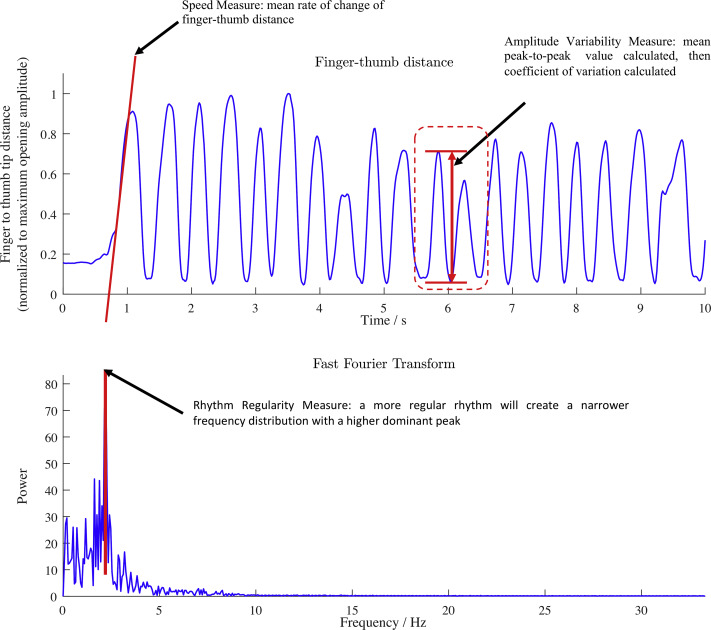
\includegraphics[width=1\textwidth]{grafica}
	\caption[Gráficas donde se visualiza la obtención de la velocidad, de la amplitud y del ritmo.]{Gráficas donde se visualiza la obtención de la velocidad y de la amplitud (arriba) y la obtención del ritmo (abajo)~\cite{goetz2008mds}.}
	\label{fig:grafica}
\end{figure}

Finalmente, se analizaron los datos y se obtuvieron conclusiones positivas ya que las diferencias de una persona que padece Parkinson de otra que no son notorias en este tipo de movimientos.

El experimento de este proyecto se realizó con 138 manos, tanto derecha como izquierda, de los cuales 39 tenían Parkinson y 30 no.

\subsection{A computer vision framework for finger-tapping evaluation in Parkinson's disease}
Este proyecto~\cite{khan2014computer} trata de identificar el Parkinson mediante el movimiento de la pinza, pero añadiendo además un reconocimiento facial, con el cual mejorar la obtención de los datos.

Para ello, se siguió el diagrama que se observa en la figura \ref{fig:diagramacara} con los siguientes pasos:
 
\begin{enumerate}
	\item Detectar la cara de la persona mediante un rectángulo y las dos regiones donde está cada mano. 
	\item Recoger las coordenadas del movimiento de las manos mediante el dedo índice. 
	\item Normalizar las coordenadas respecto al rectángulo que recuadra la cara de la persona. 
	\item Extraer las características de cada apertura y cierre de la pinza. 
	\item Realizar una clasificación utilizando una máquina de soporte vectorial (SVM) para clasificar los niveles de la enfermedad.
\end{enumerate}

\begin{figure}[h]
	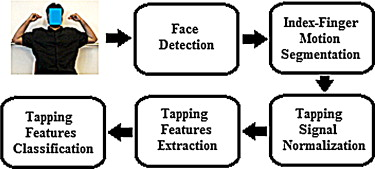
\includegraphics[width=1\textwidth]{diagrama_cara}
	\caption[Pasos que se siguieron para la realización de este proyecto.]{Pasos que se siguieron para la realización de este proyecto~\cite{khan2014computer}.}
	\label{fig:diagramacara}
\end{figure}

El paso de la detección de la cara está basado en que el tamaño de la mano de una persona adulta es muy parecido a la altura de su cara, por lo que se puede realizar una normalización de los datos obtenidos de la mano con respecto a la cara, la cual se realiza en el tercer paso, para así tener en cuenta la distancia a la que está la cámara y que no afecte al resultado. Por otro lado, se detectan a la vez las manos para poder procesarlas en los pasos posteriores. Para esta detección, se utilizó la biblioteca OpenCV.

Para el siguiente paso, el de la detección del movimiento de los dedos, se realiza un análisis de la diferencia entre los cuatro fotogramas anteriores y los 4 posteriores para conocer el movimiento de las manos, ambas de forma separada, tal y como se aprecia en la figura \ref{fig:procesamientomanos}. Para que exista movimiento, se considera que tiene que haber una diferencia absoluta de 40 píxeles o más, ya que menos representa movimiento insignificante.

\begin{figure}[h]
	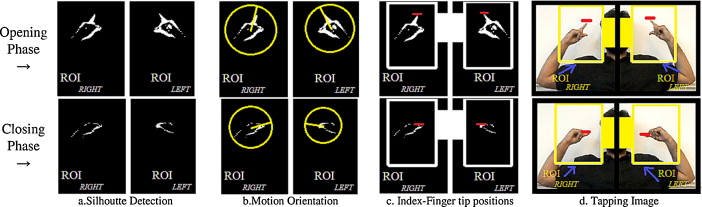
\includegraphics[width=1\textwidth]{procesamiento_manos}
	\caption[Detección de la silueta de cada mano, orientación del movimiento, posiciones del los dedos índice y la imagen actual.]{Detección de la silueta de cada mano (a), orientación del movimiento (b), posiciones del los dedos índice (c) y la imagen actual (d)~\cite{khan2014computer}.}
	\label{fig:procesamientomanos}
\end{figure}

Una vez obtenidos las coordenadas del movimiento del paso anterior, en el tercer paso, estas se calibran utilizando la cara de la persona, para normalizar los datos y que no varíen de la distancia a la cámara. Para comprobar que el algoritmo de normalización estaba ajustando correctamente los valores, se realizó una comparación del algoritmo con la utilización de marcadores de color rojo puestos en los dedos, dando el resultado que se aprecia en la figura \ref{fig:comparacioncara}. Estos marcadores de color rojo, fueron procesados con el espacio HSV, asegurándose además de que no hubiera ningún otro elemento rojo que pudiera interferir.

\begin{figure}[h]
	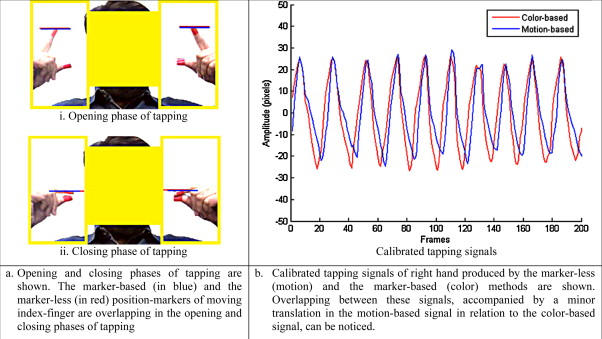
\includegraphics[width=1\textwidth]{comparacion_cara}
	\caption[Marcadores rojos y comparación del algoritmo y el procesado de los marcadores.]{Marcadores rojos puestos en los dedos para detectar la distancia (a) y comparación del algoritmo (azul) y el procesado de los marcadores (rojo) para conocer si el algoritmo ajustaba correctamente (b)~\cite{khan2014computer}.}
	\label{fig:comparacioncara}
\end{figure}

En el penúltimo paso, se extraen a partir de las coordenadas normalizadas del apartado anterior características para poder realizar una clasificación. Hubo que tener en cuenta que, generalmente, las mujeres realizan el movimiento de forma más lenta que los hombres, al igual que sucede con la mano dominante y la no dominante, pues la primera es más rápida. Las características más importantes que se extrajeron fueron: velocidad, amplitud, ritmo y comparación entre franjas horarias.

En el último paso, estas características fueron utilizadas para entrenar un clasificador, con el cual sea capaz de clasificar cada persona con el nivel de Parkinson según la escala UPDRS para el \textit{finger-tapping}, que es el tipo de movimiento que se utilizó en el proyecto. Una vez obtenidos el modelo con las predicciones, se analizaron y se concluyó que esta forma de detectar el Parkinson es viable, principalmente porque es más económico que otro tipo de detección, la cual puede necesitar de equipo costoso, y no requiere de una experiencia para poder utilizar el software.

Este experimento se realizó con los pacientes del centro clínico DIREQT (\textit{Duodopa Infusion: Randomized Efficacy and Quality of life Trial}). Había mezcla de sexos y las edades estaban comprendidas entre los 50 y 75 años. Cada grabación se realizó a lo largo del día a diferentes horas con el fin de poder obtener posibles diferencias dependiendo del momento del día, obteniendo 17 grabaciones de cada paciente.

\subsection{Tabla resumen}
En esta sección se recoge de manera resumida en una tabla aquellas medidas que han sido utilizadas en los trabajos expuestos anteriormente y en este TFG.

\begin{table}[h]
	\begin{center}
		\begin{tabular}{| c | c | c | c | c | c |}
			\hline
			Trabajo & Amplitud & Tiempo & Velocidad & Ritmo & Comparación \\ \hline
			R. Pereira et al.~\cite{pereira2016new} &  &  &  &  & X \\
			R. Jaber et al.~\cite{jaber2021proposing} & X & X & X & X & \\ 
			Williams et al.~\cite{williams2020discerning} & X & & X & X & \\
			Khan et al.~\cite{khan2014computer} & X & & X & X & X \\
			Este trabajo & X & X & X &  & \\ \hline
		\end{tabular}
		\caption{Tabla que resume las medidas utilizadas para detectar el Parkinson.}
		\label{tab:medidas}
	\end{center}
\end{table}

		\capitulo{7}{Conclusiones y Líneas de trabajo futuras}
 En este apartado, se exponen las conclusiones obtenidas tras realizar el trabajo. Además, se comentan las posibles líneas futuras del proyecto.
 
 \section{Conclusiones}
 Como ya se ha comentado en el punto \ref{resultados} de la sección de aspectos relevantes, se ha obtenido un clasificador capaz de realizar una clasificación bastante aceptable. Además, los objetivos planteados al inicio del proyecto se han podido completar en su totalidad o en gran parte de ella.
 
 \subsection{Objetivo de la investigación}
 Este objetivo ha podido ser completado satisfactoriamente, ya que se ha realizado una fase de investigación sobre la inteligencia artificial, concretamente, de la visión artificial.
 
 Se han podido realizar procesamientos de manos de personas tanto con Parkinson como sin Parkinson para obtener características suficientemente buenas como para identificar aquellas personas que padecen la enfermedad.
 
 Además, se han trabajado con diferentes modelos para probar cómo de eficaz es cada algoritmo para realizar una correcta predicción.
 
 \subsection{Objetivo de la aplicación web}
 Este objetivo también ha podido ser completado satisfactoriamente.
 
 La aplicación es totalmente funcional, ya que cuenta con varias opciones de administración, además de una pantalla amigable y sencilla para ser utilizada sin requerir conocimientos previos.
 
 El mayor inconveniente ha sido la clasificación. La aplicación está diseñada para predecir tres niveles de probabilidad de tener Parkinson: baja (menor al 33 \%), media (entre el 33 \% y el 67 \%) y alta (mayor al 67 \%), sin embargo, no suele llegar al nivel bajo. Teniendo en cuenta que este proyecto ha tratado una clasificación binaria (\textit{i. e.} sí tiene Parkinson o no), lo lógico sería pensar que no tener Parkinson equivale a un nivel bajo, un nivel alto equivaldría a tener Parkinson y un nivel medio sería un punto intermedio. No obstante, generalmente, es capaz de distinguir una persona con Parkinson de una que no, ya que para la primera predice entre un 80 y un 90 \%, mientras que para la segunda predice entre 40 y un 50 \%.
 
 \section{Líneas futuras}
 La dificultad de obtener suficientes datos para realizar el entrenamiento de modelos ha provocado que la aplicación web se haya implementado con un modelo que no es el modelo ideal, con el que diferenciar correctamente los tres niveles de probabilidad de padecer Parkinson, ya que el modelo actual apenas realiza predicciones con un bajo porcentaje.
 
 Sin embargo, dada la sencillez para cambiar el modelo de predicción de la aplicación, pues se ha implementado una opción de configuración para poder cambiar rápidamente el modelo, como línea futura se puede proponer entrenar un mejor clasificador utilizando datos mejores para poder utilizarlo en la aplicación.
 
 Además, este trabajo se ha centrado en 7 clasificadores, pero puede extenderse utilizando más clasificadores que podrían realizar mejores predicciones, teniendo en cuenta que hay otros métodos y clasificadores más complejos. Los clasificadores utilizados también se han visto afectados por los datos utilizados, ya que uno de los clasificadores que se han utilizado podría verse beneficiado si se entrenase con datos de mayor calidad. 
 
 En cuanto a los datos utilizados, se podría realizar un estudio con un mayor número de datos de mayor calidad para poder realizar un mejor entrenamiento de clasificadores. Los datos utilizados en este trabajo no estaban estandarizados, es decir, cada persona realizaba unos movimientos que podían afectar a la hora de clasificar. Por ejemplo, si todos realizasen los movimientos a la mayor velocidad que pudieran, o abriesen la pinza lo mayor posible, se conseguiría una mejor diferencia para poder obtener distinciones entre las clases, pues teóricamente una persona sana podrá realizar los movimientos con menor dificultad que una persona enferma. Si no se realiza una estandarización de los movimientos, podría ocurrir que una persona con Parkinson haga el movimiento más rápido que una persona sana, debido a que la segunda podría realizar el movimiento de forma lenta, aun pudiendo aumentar la velocidad.
 
 Otra de las posibles líneas futuras podría ser obtener otras características como el ritmo o la aceleración del movimiento. Esto podría mejorar la clasificación, ya que se podría obtener un patrón que fuese más eficaz para identificar el Parkinson que las características utilizadas en este trabajo.

		
		
		\bibliographystyle{plain}
		\bibliography{bibliografia}
		
	\end{document}
